% Self-contained: this file writes refs.bib on compile and inlines Figure 4.
\begin{filecontents*}[overwrite]{refs.bib}
@inproceedings{leviathan2023speculative,
  title={Fast Inference from Transformers via Speculative Decoding},
  author={Leviathan, Yaniv and Kalman, Matan and Matias, Yossi},
  booktitle={ICML},
  year={2023}
}

@inproceedings{chen2023accelerating,
  title={Accelerating Large Language Model Decoding with Speculative Sampling},
  author={Chen, Charlie and Borgeaud, Sebastian and Irving, Geoffrey and Lespiau, Jean-Baptiste and Sifre, Laurent and Jumper, John},
  booktitle={arXiv:2302.01318},
  year={2023}
}

@article{cai2024medusa,
  title={{Medusa}: Simple {LLM} Inference Acceleration Framework with Multiple Decoding Heads},
  author={Cai, Tianle and Li, Yuhong and Geng, Zhengyang and Peng, Hongwu and Lee, Jason D. and Chen, Deming and Dao, Tri},
  journal={arXiv:2401.10774},
  year={2024}
}

@article{li2024eagle,
  title={{EAGLE}: Speculative Sampling Requires Rethinking Feature Uncertainty},
  author={Li, Yuhui and Wei, Fangyun and Zhang, Chao and Zhang, Hongyang},
  journal={arXiv:2401.15077},
  year={2024}
}

@article{yang2024gateddelta,
  title={Gated Delta Networks: Improving Mamba2 with Delta Rule},
  author={Yang, Songlin and Wang, Bailin and Zhang, Yu and Shen, Yikang and Kim, Yoon},
  journal={arXiv:2412.06464},
  year={2024}
}

@article{gu2023mamba,
  title={Mamba: Linear-Time Sequence Modeling with Selective State Spaces},
  author={Gu, Albert and Dao, Tri},
  journal={arXiv:2312.00752},
  year={2023}
}

@article{qwen3,
  title={{Qwen3} Technical Report},
  author={{Qwen Team}},
  journal={arXiv:2505.09388},
  year={2025}
}

@misc{qwen38card,
  title={{Qwen3.8-27B} Model Card},
  author={{Qwen Team}},
  howpublished={Hugging Face},
  year={2026},
  note={https://huggingface.co/Qwen/Qwen3.8-27B}
}

@misc{qwen35card,
  title={{Qwen3.5-27B} Model Card},
  author={{Qwen Team}},
  howpublished={Hugging Face},
  year={2026}
}

@inproceedings{kwon2023vllm,
  title={Efficient Memory Management for Large Language Model Serving with {PagedAttention}},
  author={Kwon, Woosuk and Li, Zhuohan and Zhuang, Siyuan and Sheng, Ying and Zheng, Lianmin and Yu, Cody Hao and Gonzalez, Joseph E. and Zhang, Hao and Stoica, Ion},
  booktitle={SOSP},
  year={2023}
}

@article{zheng2024sglang,
  title={{SGLang}: Efficient Execution of Structured Language Model Programs},
  author={Zheng, Lianmin and Yin, Liangsheng and Xie, Zhiqiang and Sun, Chuyue and Huang, Jeff and Yu, Cody Hao and Cao, Shiyi and Kozyrakis, Christos and Stoica, Ion and Gonzalez, Joseph E. and Barrett, Clark and Sheng, Ying},
  journal={arXiv:2312.07104},
  year={2024}
}

@inproceedings{zhong2024distserve,
  title={{DistServe}: Disaggregating Prefill and Decoding for Goodput-optimized Large Language Model Serving},
  author={Zhong, Yinmin and Liu, Shengyu and Chen, Junda and Hu, Jianbo and Zhu, Yibo and Liu, Xuanzhe and Jin, Xin and Zhang, Hao},
  booktitle={OSDI},
  year={2024}
}

@article{lin2024qserve,
  title={{QServe}: {W4A8KV4} Quantization and System Co-design for Efficient {LLM} Serving},
  author={Lin, Yujun and Tang, Haotian and Yang, Shang and Zhang, Zhekai and Xiao, Guangxuan and Gan, Chuang and Han, Song},
  journal={arXiv:2405.04532},
  year={2024}
}

@misc{mlx2023,
  title={{MLX}: Efficient Machine Learning on {Apple} Silicon},
  author={Hannun, Awni and others},
  howpublished={https://github.com/ml-explore/mlx},
  year={2023}
}

@misc{mlxlm,
  title={{mlx-lm}},
  author={{MLX Contributors}},
  howpublished={https://github.com/ml-explore/mlx-lm},
  year={2024}
}

@misc{mlxlm990,
  title={Native {MTP} speculative decoding ({Qwen3.5}/{3.6} reference implementation)},
  author={{mlx-lm contributors}},
  howpublished={GitHub Pull Request 990},
  year={2026}
}

@misc{mlxvlm,
  title={{mlx-vlm}},
  author={Blaizzy and others},
  howpublished={https://github.com/Blaizzy/mlx-vlm},
  year={2024}
}

@misc{mlxvlm1423,
  title={Chunked {Gated DeltaNet} prefill},
  author={{mlx-vlm contributors}},
  howpublished={GitHub Pull Request 1423},
  year={2026}
}

@misc{mlxvlm945,
  title={Per-chunk \texttt{mx.eval} and \texttt{clear\_cache} stall},
  author={{mlx-vlm contributors}},
  howpublished={GitHub Issue 945},
  year={2026}
}

@misc{omlx2874,
  title={Optimal Configuration for {Qwen3.8-27B} on {M3 Max} 128{GB}},
  author={taozhiyuai and others},
  howpublished={oMLX Issue 2874},
  year={2026}
}

@misc{omlx2781,
  title={{Qwen} {ANE} Prompt Processing on {M3 Max}},
  author={{oMLX contributors}},
  howpublished={oMLX Issue 2781},
  year={2026}
}

@misc{weschera2026,
  title={{Qwen} 3.8 27{B} on {Apple} Silicon: 53--72 tok/s with {oMLX} {ANE} + native {MTP}},
  author={Weschera},
  howpublished={https://github.com/Weschera/Qwen3.8-27B-oMLX-MTP-Mac},
  year={2026}
}

@misc{ollama019,
  title={{Ollama} is now powered by {MLX} on {Apple} Silicon in preview},
  author={{Ollama}},
  howpublished={https://ollama.com/blog/mlx},
  year={2026},
  month={March}
}

@article{frantar2023gptq,
  title={{GPTQ}: Accurate Post-Training Quantization for Generative Pre-trained Transformers},
  author={Frantar, Elias and Ashkboos, Saleh and Hoefler, Torsten and Alistarh, Dan},
  journal={ICLR},
  year={2023}
}

@article{lin2024awq,
  title={{AWQ}: Activation-aware Weight Quantization for {LLM} Compression and Acceleration},
  author={Lin, Ji and Tang, Jiaming and Tang, Haotian and Yang, Shang and Chen, Wei-Ming and Wang, Wei-Chen and Xiao, Guangxuan and Dang, Xingyu and Gan, Chuang and Han, Song},
  booktitle={MLSys},
  year={2024}
}

@article{xiao2024smoothquant,
  title={{SmoothQuant}: Accurate and Efficient Post-Training Quantization for Large Language Models},
  author={Xiao, Guangxuan and Lin, Ji and Seznec, Mickael and Wu, Hao and Demouth, Julien and Han, Song},
  booktitle={ICML},
  year={2023}
}

@article{yuan2024specprefill,
  title={{SpecPrefill}: Accelerating {LLM} Prefill with Speculative Decoding},
  author={Yuan and others},
  journal={arXiv},
  year={2025}
}

@article{swiftkv,
  title={{SwiftKV}: Fast Prefill-Optimized Inference with Knowledge-Preserving Layer Skipping},
  author={Agarwal and others},
  journal={arXiv},
  year={2025}
}

@article{pyramidkv,
  title={{PyramidKV}: Dynamic {KV} Cache Compression based on Pyramidal Information Funneling},
  author={Cai and others},
  journal={arXiv:2406.02069},
  year={2024}
}

@inproceedings{dao2022flashattention,
  title={{FlashAttention}: Fast and Memory-Efficient Exact Attention with {IO}-Awareness},
  author={Dao, Tri and Fu, Daniel Y. and Ermon, Stefano and Rudra, Atri and R{\'e}, Christopher},
  booktitle={NeurIPS},
  year={2022}
}

@article{shazeer2017moe,
  title={Outrageously Large Neural Networks: The Sparsely-Gated Mixture-of-Experts Layer},
  author={Shazeer, Noam and Mirhoseini, Azalia and Maziarz, Krzysztof and Davis, Andy and Le, Quoc and Hinton, Geoffrey and Dean, Jeff},
  journal={arXiv:1701.06538},
  year={2017}
}

@article{fedus2022switch,
  title={Switch Transformers: Scaling to Trillion Parameter Models with Simple and Efficient Sparsity},
  author={Fedus, William and Zoph, Barret and Shazeer, Noam},
  journal={JMLR},
  year={2022}
}

@article{huang2024llm,
  title={A Survey on Efficient Inference for Large Language Models},
  author={Zhou, Zixuan and others},
  journal={arXiv:2404.14294},
  year={2024}
}

@misc{llamacpp,
  title={{llama.cpp}},
  author={Gerganov, Georgi and contributors},
  howpublished={https://github.com/ggerganov/llama.cpp},
  year={2023}
}

@misc{qwen31826,
  title={Chat template injects empty think tags under \texttt{enable\_thinking=false}},
  author={{QwenLM contributors}},
  howpublished={Qwen3 Issue 1826},
  year={2026}
}

@misc{mlxengine176,
  title={Prefix cache miss from {Qwen} generation-prompt think tags},
  author={{LM Studio mlx-engine contributors}},
  howpublished={mlx-engine Issue 176},
  year={2026}
}

@misc{mlxlm1077,
  title={{GDN} cache slice leak},
  author={{mlx-lm contributors}},
  howpublished={Issue 1077},
  year={2026}
}

@misc{mlxlm1162,
  title={{KVCache} offset not restored from keys},
  author={{mlx-lm contributors}},
  howpublished={Issue 1162},
  year={2026}
}

@misc{mlx3350,
  title={Small Metal free-cache forces per-layer malloc},
  author={{MLX contributors}},
  howpublished={mlx Issue 3350},
  year={2026}
}

@misc{vllm36649,
  title={\texttt{mamba\_cache\_mode=all} for hybrid {APC}},
  author={{vLLM contributors}},
  howpublished={vLLM Issue 36649},
  year={2026}
}

@inproceedings{pope2023efficiently,
  title={Efficiently Scaling Transformer Inference},
  author={Pope, Reiner and Douglas, Sholto and Chowdhery, Aakanksha and Devlin, Jacob and Bradbury, James and Heek, Jonathan and Xiao, Kefan and Agrawal, Shivani and Dean, Jeff},
  booktitle={MLSys},
  year={2023}
}

@article{patel2024splitwise,
  title={{Splitwise}: Efficient Generative {LLM} Inference Using Phase Splitting},
  author={Patel, Pratyush and Choukse, Esha and Zhang, Chaojie and Goiri, {\'I}{\~n}igo and Warrier, Brijesh and Mahalingam, Nithish and Bianchini, Ricardo},
  booktitle={ISCA},
  year={2024}
}

@misc{appleum,
  title={Unified Memory Architecture},
  author={{Apple}},
  howpublished={Apple Silicon documentation},
  year={2020}
}

@misc{stared2026,
  title={Benching local {LLMs} on {Apple} Silicon},
  author={stared},
  howpublished={https://github.com/stared/benching-local-llms-on-apple-silicon},
  year={2026}
}

@misc{terminalbytes2026,
  title={Run {Qwen3.8} 27{B} locally: real numbers from my {Mac} {Studio}},
  author={{TerminalBytes}},
  year={2026},
  howpublished={Community bench of Ollama Q4\_K\_M Qwen3.8-27B vs.\ Qwen3.6-27B on M3 Ultra}
}

@misc{orcarouter2026,
  title={{Qwen3.8-27B} on {Apple} Silicon: {MLX} Setup, {VRAM} and Reality},
  author={{OrcaRouter}},
  year={2026},
  howpublished={https://huggingface.co/orcarouter/Qwen3.8-27B-MLX}
}

@misc{ctaylor83mtp,
  title={{Qwen3.8-27B} {MTP}: the flag was free the whole time},
  author={ctaylor83},
  howpublished={https://github.com/ctaylor83/qwen38-mtp},
  year={2026}
}

@misc{zlabdflash,
  title={{DFlash2} draft models for {Qwen3.8}},
  author={{z-lab}},
  howpublished={Hugging Face},
  year={2026}
}

@article{yarn2024,
  title={{YaRN}: Efficient Context Window Extension of Large Language Models},
  author={Peng, Bowen and Quesnelle, Jeffrey and Fan, Honglu and Shippole, Enrico},
  journal={ICLR},
  year={2024}
}

@inproceedings{vaswani2017attention,
  title={Attention Is All You Need},
  author={Vaswani, Ashish and Shazeer, Noam and Parmar, Niki and Uszkoreit, Jakob and Jones, Llion and Gomez, Aidan N. and Kaiser, {\L}ukasz and Polosukhin, Illia},
  booktitle={NeurIPS},
  year={2017}
}

@article{dao2024flashattn2,
  title={{FlashAttention-2}: Faster Attention with Better Parallelism and Work Partitioning},
  author={Dao, Tri},
  journal={ICLR},
  year={2024}
}

@misc{slotbankrepo,
  title={slotbank},
  author={Heid, Andre},
  howpublished={https://github.com/Andylol111/slotbank},
  year={2026}
}

@article{mixtral2024,
  title={Mixtral of Experts},
  author={Jiang, Albert Q. and others},
  journal={arXiv:2401.04088},
  year={2024}
}

@inproceedings{rajbhandari2022deepspeed,
  title={{DeepSpeed-MoE}: Advancing Mixture-of-Experts Inference and Training to Power Next-Generation {AI} Scale},
  author={Rajbhandari, Samyam and others},
  booktitle={ICML},
  year={2022}
}

@inproceedings{he2022fastermoe,
  title={{FasterMoE}: Modeling and Optimizing Training of Large-scale Dynamic Pre-trained Models},
  author={He, Jiaao and others},
  booktitle={PPoPP},
  year={2022}
}

@article{cai2024medusafull,
  title={{Medusa}: Simple {LLM} Inference Acceleration Framework with Multiple Decoding Heads},
  author={Cai, Tianle and others},
  journal={arXiv:2401.10774},
  year={2024}
}

@misc{gemfilter,
  title={{GemFilter}: Training-Free Token Filtering for Efficient {LLM} Prefill},
  author={Anonymous},
  year={2025}
}

@misc{pflash,
  title={{PFlash}: Dropping Prompt Tokens for Faster Prefill},
  author={Anonymous},
  year={2025}
}

@article{xiao2024infllm,
  title={{InfLLM}: Training-Free Long-Context Extrapolation for {LLMs} with an Efficient Context Memory},
  author={Xiao, Chaojun and others},
  journal={arXiv:2402.04617},
  year={2024}
}

@inproceedings{dao2022flashattention2,
  title={{FlashAttention}: Fast and Memory-Efficient Exact Attention with {IO}-Awareness},
  author={Dao, Tri and Fu, Daniel Y. and Ermon, Stefano and Rudra, Atri and R{\'e}, Christopher},
  booktitle={NeurIPS},
  year={2022}
}

@misc{mlxswift225,
  title={asyncEval prefill pipeline on {M5 Max} vs {M2 Mini}},
  author={{mlx-swift-lm contributors}},
  howpublished={GitHub Issue 225},
  year={2026}
}

@misc{mlxnode68,
  title={Chunked {GDN} slower than per-step on Metal},
  author={{mlx-node contributors}},
  howpublished={GitHub Issue 68},
  year={2026}
}

@misc{sglang12867,
  title={{GDN} radix cache at \texttt{page\_size>1}},
  author={{SGLang contributors}},
  howpublished={sgl-project/sglang\#12867},
  year={2026}
}

@misc{atomgradient,
  title={{Qwen3.5-9B} Metal prefill breakdown},
  author={atomgradient},
  howpublished={mlx-inference-bench},
  year={2026}
}

@misc{nathanmaine,
  title={{Qwen3.8-27B} {MTP} on {M5 Max} 128{GB}},
  author={NathanMaine},
  year={2026},
  howpublished={https://github.com/NathanMaine/qwen-mlx-offline}
}

@misc{olmoe,
  title={{OLMoE}: Open Mixture-of-Experts Language Models},
  author={Muennighoff, Niklas and others},
  journal={arXiv:2409.02060},
  year={2024}
}

@misc{applejetsam,
  title={Responding to Low-Memory Warnings on {iOS} and {macOS} (jetsam)},
  author={{Apple}},
  howpublished={Apple Developer Documentation},
  year={2023},
  note={https://developer.apple.com/documentation/xcode/investigating-memory-access-crashes}
}

@misc{mlxlmcache,
  title={\texttt{trim\_prompt\_cache} and \texttt{can\_trim\_prompt\_cache}},
  author={{MLX Contributors}},
  howpublished={mlx-lm \texttt{models/cache.py}},
  year={2025},
  note={https://github.com/ml-explore/mlx-lm}
}

@misc{qwen35a3b,
  title={{Qwen3.5-35B-A3B} Model Card},
  author={{Qwen Team}},
  howpublished={Hugging Face},
  year={2026}
}

@misc{applemetalws,
  title={{Metal} resource limits and recommended working-set size},
  author={{Apple}},
  howpublished={Metal Programming Guide},
  year={2024}
}
\end{filecontents*}

\documentclass[11pt]{article}

\usepackage[margin=1in]{geometry}
\usepackage{times}
\usepackage{amsmath,amssymb,amsthm}
\usepackage{booktabs}
\usepackage{graphicx}
\usepackage{xcolor}
\usepackage{tikz}
\usetikzlibrary{arrows.meta,positioning,fit,calc,shapes.geometric,patterns}
\usepackage{algorithm}
\usepackage{algpseudocode}
\usepackage{hyperref}
\usepackage{natbib}
\usepackage{enumitem}
\usepackage{caption}
\usepackage{subcaption}
\usepackage{titlesec}
\usepackage{fancyhdr}
\usepackage{microtype}
\usepackage{url}
\usepackage{setspace}
\usepackage{longtable}
\usepackage{array}
\usepackage{multirow}

\hypersetup{
  colorlinks=true,
  linkcolor=black,
  citecolor=black,
  urlcolor=blue,
  pdftitle={slotbank: Hybrid-Safe Local Serving of Dense and Mixture-of-Experts Language Models on 24 GB Unified Memory},
  pdfauthor={Andre Heid},
  pdfsubject={Systems manuscript on local Qwen3.8-27B serving on a 24 GB Apple M4 Air},
  pdfkeywords={on-device LLM serving, Apple Silicon, unified memory, Gated DeltaNet, speculative decoding, prefix caching, mixture of experts, reproducibility}
}

\pagestyle{fancy}
\fancyhf{}
\fancyhead[L]{\small slotbank Systems Manuscript}
\fancyhead[R]{\small Heid, 2026}
\fancyfoot[C]{\thepage}
\renewcommand{\headrulewidth}{0.4pt}

\theoremstyle{definition}
\newtheorem{definition}{Definition}
\newtheorem{proposition}{Proposition}
\newtheorem{remark}{Remark}

\newcommand{\slotbank}{\textsc{slotbank}}
\newcommand{\gdn}{Gated DeltaNet}
\newcommand{\tokspersec}{\mathrm{tok/s}}

\title{\vspace{-1.2em}
\textbf{slotbank}: Hybrid-Safe Local Serving of Dense and Mixture-of-Experts\\
Language Models on 24\,GB Unified Memory\\[0.4em]
\large Running Qwen3.8-27B on a Fanless Apple M4 Air}

\author{
Andre Heid\\
Yale University\\
\texttt{andre.h.costa@yale.edu}
}

\date{2 September 2026 \\[0.3em] \small Technical report (companion to \texttt{main.tex}, the conference extract)}

\begin{document}
\maketitle
\thispagestyle{fancy}

\begin{abstract}
This report describes how I run Qwen3.8-27B, and a handful of larger Mixture-of-Experts checkpoints, on a fanless 24\,GB Apple M4 Air. Finding a 4-bit pack is easy. The hard part is keeping the emitted tokens identical to the target model while the same DRAM is asked to hold the Metal working set, the file cache, and an agent prompt that was written for a hosted API.

\slotbank{} is a single-process MLX runtime. When an MoE expert bank will not fit in the Metal working set, stacked Switch-linear weights are moved to a file-backed bank and a resident pack of $C$ slots, so \texttt{gather\_qmm} only ever sees the pack. Dense 27B has no useful expert subset; the same idea reduces to fitting an affine-4 pack plus a 66.4M multi-token-prediction sidecar in an 18\,GiB working set (\texttt{--leave-free 6g}) and calling stock \texttt{mlx-vlm}. Speculative decode uses that sidecar with Leviathan--Chen rejection sampling and \texttt{rollback\_speculative\_cache}. Prefill is tiled in process, with an exact-prefix snapshot cache. Gated DeltaNet state is never trimmed.

Several published accelerations do not apply here, or apply only in a form that changes the text. Hybrid caches are untrimmable; \texttt{mlx-lm}'s speculative rewind is a no-op on that path and does not raise; Qwen's chat template inserts generation-prompt tokens that are not a prefix of the next agent encode; Neural Engine prefill figures above ${+}200\%$ were measured on 64--128\,GB machines that keep a second weight copy. Those observations are recorded in a small catalog with unit tests, and the admission, envelope, and context-log code is kept free of MLX so the policy can be checked without pinning 15\,GiB.

On this Air I measured 5.71 tok/s greedy, 13.47 / 9.95 tok/s with native MTP (count / code), about 48 tok/s on a cold 819-token prefill, and $19\times$ lower time-to-first-token when the next request is an exact prefix. Bandwidth-scaled Metal numbers from an M3 Max sit close to those decode rates. I do not have a 40--70 tok/s 27B on 120\,GB/s; that class of result uses more cores, more bandwidth, and usually a second residency I cannot afford.

A dated verification campaign (\S\ref{sec:verify}, campaign \texttt{20260902T001357Z}) maps twenty-four claims to tests. Twenty-one are reproduced on a Linux host with no Metal weights; two Air clocks are pin-checked; two gaps (envelope task quality, fanless soak) are named so they cannot be promoted to results. The filtered pytest tree on that host is 221 passed / 23 skipped. The envelope suite is 29 OMP-shaped prompts and is a structural oracle, not a quality study.
\end{abstract}

\vspace{0.4em}
\noindent\textbf{Keywords:} on-device LLM serving, Apple Silicon, unified memory, Gated DeltaNet, speculative decoding, prefix caching, mixture of experts, agent harnesses

\tableofcontents
\vspace{1em}

%======================================================================
\section{Introduction}
\label{sec:intro}

Qwen3.8-27B is available as a downloadable checkpoint~\citep{qwen38card}. A 4-bit pack is about 15\,GiB, which will load on a 24\,GB MacBook Air if little else is wired. That observation is often treated as the end of the story. In practice the same machine is also asked to hold an Oh My Pi (OMP) harness of 26k--39k tokens, and several published ``Mac speedups'' assume a Neural Engine procedure bank or a second Core ML copy of the MLPs. Those extra residencies do not fit next to the 15\,GiB pack. Hybrid Gated DeltaNet state cannot be paged the way a transformer KV cache can, so the usual 128k tricks are not available either.

I wrote this as a systems account of one working setup: what is resident, which optimizations I kept after they met a 48+16 hybrid, where existing libraries were silently wrong, and which 2026 ideas I tried or refused. All measurements that are not cited to someone else come from a fanless M4 Air, 24\,GB unified memory, roughly 10 GPU cores, 120\,GB/s. The line I actually leave running is
\begin{quote}
\texttt{slotbank serve --model Qwen3.8-27B-4bit --leave-free 6g --thinking --vision --direct}
\end{quote}
with \texttt{Qwen3.8-27B-MTP-4bit} attached if I omit \texttt{--draft}. Thinking and vision stay on for daily use. I turn them off only when I want a decode ceiling.

\subsection{Constraints I would not trade for tok/s}

I did not start from a search for peak throughput. I started from a short list of things I was unwilling to break.

\begin{enumerate}[leftmargin=1.4em,itemsep=0.25em]
\item Daily serve is the 27B. I do not swap Qwen3.5-4B in, use 4B as a 27B drafter, or skip full-attention layers while drafting.
\item Speculative tokens have to be tokens the 27B would have produced at the requested temperature. That is Leviathan--Chen rejection sampling~\citep{leviathan2023speculative,chen2023accelerating} through \texttt{mlx-vlm}'s \texttt{generate\_step} and \texttt{rollback\_speculative\_cache}.
\item Qwen3.8-27B is 64 layers in a $3{:}1$ pattern: 48 \gdn{} layers with $O(1)$ recurrent state and 16 full-attention layers at about 64\,KiB/token. \texttt{can\_trim\_prompt\_cache} is false. I do not page, LRU, or trim that cache.
\item OMP still sends a full cloud harness. The local envelope condenses what Metal prefills. I do not edit OMP YAML to make the model look faster.
\item One Metal worker. MLX arrays do not travel between threads. There is no draft/verify queue pair, no prefill/decode split~\citep{zhong2024distserve}, and no second process holding another copy of the weights.
\end{enumerate}

The list is a reaction to a bug I hit early. \texttt{mlx-lm}'s \texttt{speculative\_generate\_step} rewinds rejected drafts with \texttt{trim\_prompt\_cache}. On \texttt{ArraysCache} that call is a no-op. Later tokens are then conditioned on drafts that were never printed, and nothing is raised~\citep{slotbankrepo}. Turning speculation on for Qwen3.5/3.8 through that entry point does not make the model faster. It makes a different, unlabeled model.

\subsection{Problem statement and research questions}
\label{sec:rqs}

The systems problem is this. Serve Qwen3.8-27B-4bit, and when needed a 35B-A3B expert bank, on one 24\,GB fanless Air, such that (i)~emitted tokens remain the target model's at the requested sampler, (ii)~an OMP-sized dump does not jetsam or HTTP-400, and (iii)~a follow-up encode that really is a prefix hits PrefixCache. The machine is the experimental unit. I do not have a second Air, a Max, or a cluster.

I treat five questions as the conference-shaped core. Everything else in the report is support, refusal, or operational colour.

\begin{enumerate}[leftmargin=1.8em,itemsep=0.35em]
\item[\textbf{RQ1}] On this Air, what named clocks does 27B-4bit actually hit, and how do they sit against bandwidth-scaled Max numbers and the 2026 ${+}200\%$ Mac headline? (\S\ref{sec:eval}, \S\ref{sec:mac200}; claims \texttt{C-clocks}, \texttt{C-pack-ceil}, \texttt{C-mac200}, \texttt{C-scale}.)
\item[\textbf{RQ2}] Can speculative decode raise tok/s without changing 27B text when 48/64 layers are untrimmable Gated DeltaNet? (\S\ref{sec:spec}; \texttt{C-hybrid-kv}, \texttt{C-trained-k}, \texttt{C-session}, \texttt{C-sampling}.)
\item[\textbf{RQ3}] What leave-free and slot-capacity rules admit 27B plus sidecar, or 35B-A3B experts, without treating the page cache as VRAM? (\S\ref{sec:dense}, \S\ref{sec:moe}; \texttt{C-leave-free}, \texttt{C-slots-c}.)
\item[\textbf{RQ4}] Can admission, catalog, and OMP policy be checked on a machine that cannot pin 15\,GiB, and do those checks refuse routes that change tokens? (\S\ref{sec:catalog}, \S\ref{sec:impl}; \texttt{C-fence}, \texttt{C-catalog}.)
\item[\textbf{RQ5}] Does the local envelope keep system $\le 256$, packed ids $\le 8192$, and a history-stable prefix on OMP-shaped dumps, without claiming task quality? (\S\ref{sec:envelope}, \S\ref{sec:suite}; \texttt{C-sys-cap}--\texttt{C-suite}; gap \texttt{C-quality}.)
\end{enumerate}

A sixth question---how the serve feels after a soak---is answered only as an operational note (\S\ref{sec:ops}) and as gap \texttt{C-soak}. I did not retime it on this campaign host.

\subsection{Two models, one door}

\slotbank{} began as a Mixture-of-Experts (MoE) runtime for checkpoints whose expert bank exceeds the Metal working set~\citep{shazeer2017moe,fedus2022switch}. On this Air, Qwen3.5-35B-A3B at 4-bit is 19.02\,GiB of weights, 16.9\,GiB of them experts. llama.cpp at matching quality cannot run. Stock \texttt{mlx-lm} thrashes at 0.005 tok/s. \slotbank{} with $C{=}32$ resident slots reports 4.2 cold end-to-end tok/s to 256 tokens and 6.1 warm sustained decode, with $\approx 3.8$\,GiB wired.

Dense Qwen3.8-27B has no expert subset. The same principle applies: shrink the bytes that must stay hot until they fit, then use stock kernels. Layer-streaming GDN from SSD is the fallback if even 3-bit out-of-memory-kills the process; it was not needed. Daily 27B is 4-bit plus a 66.4M-parameter MTP sidecar ($\approx 239$\,MB), not a second 15\,GiB language model.

\subsection{Contributions}

The useful parts of the work, as far as I can tell, are these.

\begin{enumerate}[leftmargin=1.4em,itemsep=0.35em]
\item A working-set model in which the $C$-slot pack and the OS page cache compete for the same DRAM. On this 24\,GB machine $C{=}32$ beat $C{=}64$ because the extra wired slots evicted the cache that was serving misses (\S\ref{sec:tiers}, \S\ref{sec:moe}).
\item Speculation that can rewind GDN: native MTP or DFlash2 through \texttt{mlx-vlm}, trained block size only, KV quantization off on the draft path, and no use of \texttt{mlx-lm} trim speculation (\S\ref{sec:spec}).
\item Prefix reuse that only restores an exact stored prefix, snapped at the pre-\texttt{/no\_think} body so Qwen's generation prompt does not poison the next encode, with KV \texttt{offset} written on restore, and a 2048-token cap after a 10k snapshot jetsamed the laptop (\S\ref{sec:prefix}).
\item An envelope that leaves OMP's YAML alone: 256-token system clip, schema-free tool names, pyramidal packing of token ids (not of GDN state), and a disk log that remains the source of truth for long context (\S\ref{sec:envelope}, \S\ref{sec:context}).
\item A catalog in \texttt{tps.py} whose tests fail if a rejected idea is marked adopted, if an adopted route needs cache trim or new target weights, and if the daily draft is no longer sidecar MTP (\S\ref{sec:catalog}, \S\ref{sec:mac200}). The same file holds a source review of the 2026 ``${+}200\%$ on Mac'' claim.
\item An import fence. Only \texttt{runtime.py}, \texttt{expert\_slots.py}, and \texttt{offload\_cache.py} may import MLX, so admission, OMP, the context log, and the catalog can be tested on a machine with no weights (\S\ref{sec:impl}).
\item A claim registry (\texttt{C-fence}{\ldots}\texttt{C-metal-toks}) and a dated campaign that records which of those claims this host can reproduce, which are Air pins, and which remain gaps (\S\ref{sec:verify}).
\end{enumerate}

I am not claiming a new attention kernel, a new quantizer, or a $3\times$ decode speedup on this Air. Figures of that size appear in 2026 Mac write-ups; \S\ref{sec:mac200} walks through which chip, which model, and which extra weight copy they used.

\subsection{Outline}

Related work is \S\ref{sec:related}. Background on unified memory, the hybrid stack, and speculation is \S\ref{sec:bg}. Design rules are \S\ref{sec:thesis}. Methods occupy \S\ref{sec:moe}--\S\ref{sec:catalog}. Implementation is \S\ref{sec:impl}. Measurement protocol is \S\ref{sec:method}. The verification campaign that binds claims to tests is \S\ref{sec:verify}. Results are \S\ref{sec:eval}, including the envelope suite (\S\ref{sec:suite}). How the serve is run day to day is \S\ref{sec:ops}. What I think is assembled versus new is \S\ref{sec:unique}. Failure modes are \S\ref{sec:threats}. Limits and closing remarks follow. The appendix lists catalog entries, the claim matrix, and a checklist for anyone citing a number.

I wrote this at technical-report length so the clocks, refusals, and campaign log sit in one artifact. The conference-shaped spine is the five RQs, the methods that answer them, the campaign, and the threats.

%======================================================================
\section{Related Work}
\label{sec:related}

\subsection{Serving systems on discrete GPUs}

vLLM's PagedAttention virtualizes the KV cache as blocks~\citep{kwon2023vllm}. SGLang adds a radix tree over prefixes~\citep{zheng2024sglang}. DistServe and Splitwise disaggregate prefill from decode across machines~\citep{zhong2024distserve,patel2024splitwise}. QServe co-designs W4A8KV4 quantization with the kernel~\citep{lin2024qserve}. All of these assume (i)~a discrete GPU with a driver-managed heap, (ii)~attention state that is a per-token tensor and can be paged, and (iii)~often a cluster. Apple unified memory inverts (i): there is no host-to-device copy to overlap, and wired Metal pages compete with the file cache. Hybrid Gated DeltaNet inverts (ii): 48 of 64 layers store a recurrent summary that cannot be sliced at a token boundary~\citep{yang2024gateddelta,gu2023mamba}. Cluster disaggregation inverts (iii): this Air is one worker.

vLLM's \texttt{mamba\_cache\_mode=all} checkpoints SSM state every block so automatic prefix caching can restore a mid-prompt hit~\citep{vllm36649}. The Metal \texttt{gated\_delta\_kernel} does not return those intermediates. Copying the vLLM API onto MLX would be a new kernel, not a wrapper.

\subsection{Speculative decoding}

Leviathan et al.\ and Chen et al.\ established lossless speculative decoding: a cheap drafter proposes $K$ tokens, the target verifies them in one forward, and rejection sampling preserves the target distribution~\citep{leviathan2023speculative,chen2023accelerating}. Medusa and EAGLE attach extra heads or a feature-level drafter~\citep{cai2024medusa,li2024eagle}. Qwen3.5/3.8 train a multi-token-prediction (MTP) head into the checkpoint~\citep{qwen3,qwen38card}. llama.cpp \texttt{draft-mtp}~\citep{ctaylor83mtp} and \texttt{mlx-lm} PR~990~\citep{mlxlm990} connect that head. DFlash2 is a distilled student with a longer trained block~\citep{zlabdflash}.

MTP itself is not the systems problem. Verify on a hybrid model has to rewind \gdn{} state. \texttt{mlx-lm} rewind uses \texttt{trim\_prompt\_cache}. \texttt{mlx-vlm} rewind uses \texttt{rollback\_speculative\_cache}. Those are not interchangeable. Prompt-lookup decoding from $n$-grams in context is implemented in \slotbank{} and is inert on Qwen3.8 because it requires a trimmable cache.

\subsection{Prefill accelerators that change the prompt}

SpecPrefill, GemFilter, SwiftKV, and PFlash skip prompt tokens or layers and quote $2$--$7\times$ time-to-first-token on CUDA~\citep{yuan2024specprefill,swiftkv}. PyramidKV compresses KV with a pyramidal keep-set~\citep{pyramidkv}. I reused the keep-set shape (sink prefix, denser early middle, tail) for \emph{which token ids are prefills}, not for recurrent state. Dropping tokens from the 27B's prompt, or distilling skip layers, is rejected: it changes the target distribution or the weights.

Chunked GDN on CUDA is a different story. \texttt{mlx-vlm} PR~1423 reports $8.5\times$ TTFT on an RTX PRO 6000 by replacing a Python $T$-loop with a chunked scan~\citep{mlxvlm1423}. The PR text states macOS/Metal is unchanged: Metal already runs \texttt{gated\_delta\_kernel} with the time loop inside the shader when $D_k \bmod 32 = 0$. Qwen3.8-27B has $D_k = D_v = 128$. Subsequent Metal measurements found the CUDA-style chunked path $2.5$--$3.5\times$ \emph{slower} than per-step on M5. The CUDA $8.5\times$ is ``ops-loop $\to$ fused,'' not ``chunked beats fused.''

\subsection{Apple Silicon runtimes}

\texttt{mlx-lm} and \texttt{mlx-vlm} are the native Metal stacks~\citep{mlx2023,mlxlm,mlxvlm}. llama.cpp ports CUDA patterns to Metal~\citep{llamacpp}. Ollama 0.19 previewed an MLX backend and published ${+}93\%$ decode on Qwen3.5-35B-A3B NVFP4, M5, 32\,GB+~\citep{ollama019}. oMLX adds ANE prefill, split procedure banks, and native MTP~\citep{omlx2874,omlx2781,weschera2026}. MTPLX is a closed-loop Mac app with custom verify kernels. Community benches on M3 Ultra show Qwen3.8-27B \emph{slower} per token than Qwen3.6-27B under Ollama Q4\_K\_M (14.0 vs.\ 28.6 tok/s) because hybrid kernels were immature~\citep{terminalbytes2026}. An M4 mini without MTP measures 5--6 tok/s~\citep{orcarouter2026}, matching this Air's greedy 5.71.

I have not found a published 24\,GB Air recipe that does all three of: survive an OMP 39k dump, keep hybrid verify exact, and hit a prefix cache on the next OMP re-encode. That intersection is what I needed, so that is what I wrote down.

\subsection{Quantization}

GPTQ, AWQ, and SmoothQuant are the standard post-training methods~\citep{frantar2023gptq,lin2024awq,xiao2024smoothquant}. \slotbank{} consumes community MLX affine-4 packs (group 64) and does not requantize. Mixed 3.5\,bpw fits and is a quality pack ($\approx 1$ tok/s on this Air). Uniform 3-bit and W8A8-style requants are rejected as a change of the 27B's weights. KV quantization is available off the draft path and forbidden on it because the verifier reads \texttt{keys.shape}.

\subsection{Mixture-of-experts serving}

The original MoE papers established that a sparse router can keep compute near that of a dense model of the active width~\citep{shazeer2017moe,fedus2022switch,mixtral2024}. Discrete-GPU serving then treated experts as a cacheable resource: DeepSpeed-MoE, FasterMoE, and Expert Parallelism shard $E$ across devices and prefetch the next hop~\citep{rajbhandari2022deepspeed,he2022fastermoe}. Those designs assume (i)~PCIe or NVLink as a copy engine that can overlap the current GEMM, (ii)~a driver heap that is not also the file cache, and (iii)~often a cluster. Unified memory inverts all three. There is no host-to-device DMA to hide; a byte that is ``on the GPU'' is a byte that is not in the page cache; and this Air is one worker. The slot pack is a capacity-limited resident window, not an Expert-Parallel replica. I size it so the rest of the bank can still live in DRAM as evictable pages.

Serving Mixtral on a 64\,GB Mac is a different problem. The bank fits, stock kernels are faster, and the remaining work is fusion. The 24\,GB case I care about is a 19\,GiB 4-bit 35B-A3B that llama.cpp would not load at matching quality. That is the MoE workload below.

\subsection{Agent harnesses versus model prompts}

Production coding agents (Claude Code, Cursor, Codex, Oh My Pi) send a cloud-sized system prompt, a tool catalog with JSON schemas, and often a working-tree dump. Hosted APIs absorb that cost in a prefix cache on a cluster. A 24\,GB laptop cannot. Most local proxies either refuse the prompt or silently truncate it. Truncation that is not a prefix of the next encode is a guaranteed cache miss and, on hybrid GDN, a full recompute. \slotbank{} treats the harness as a \emph{third object}: the agent still owns the YAML; Metal sees a condensed, cache-stable projection; disk keeps the verbatim dump. I treat that split as a product decision that happens to determine whether the prefix cache hits.

%======================================================================
\section{Background}
\label{sec:bg}

\subsection{Unified memory as three tiers}
\label{sec:tiers}

On NVIDIA, weights live in VRAM or they do not. On Apple Silicon the same physical DRAM is simultaneously the GPU heap, the CPU heap, and the file cache~\citep{appleum}. \slotbank{} names three tiers:

\begin{center}
\begin{tabular}{@{}llp{7.6cm}@{}}
\toprule
Tier & 24\,GB M4 Air & Role \\
\midrule
1 Wired Metal & $\approx 17.8$\,GiB advertised WS & Resident pack; jetsam if exceeded \\
2 Page cache & $\approx 12$--16\,GiB usable & Expert bank / mmap hits \\
3 SSD & rest & Misses via \texttt{pread} / readahead \\
\bottomrule
\end{tabular}
\end{center}

Decode throughput is bandwidth over bytes touched:
\begin{equation}
\label{eq:bw}
  \tau \;\approx\; \frac{B}{W_{\mathrm{touch}}},
\end{equation}
where $B$ is the bytes per second the serving tier can actually deliver and $W_{\mathrm{touch}}$ is the bytes read per token. On this Air, $B_{\mathrm{DRAM}} = 120$\,GB/s. A 15\,GiB 4-bit pack implies a full-pack-read ceiling
\begin{equation}
  \tau_{\mathrm{pack}} \;=\; \frac{120\times 2^{30}}{15\times 2^{30}} \;\approx\; 8\ \tokspersec.
\end{equation}
Speculative decoding can beat $\tau_{\mathrm{pack}}$ because accepted drafts amortize one target forward over several tokens. ANE prefill cannot raise $B$; it adds compute units and a second residency.

Measured I/O on the MoE path:
\begin{center}
\begin{tabular}{@{}lr@{}}
\toprule
Source & Throughput \\
\midrule
Warm page cache & $\sim 10$\,GB/s \\
SSD batched readahead & $1000$--$3300$\,MiB/s \\
SSD, one-at-a-time mmap faults & $358$\,MiB/s \\
\bottomrule
\end{tabular}
\end{center}
The last row is why \texttt{SliceStore} issues \texttt{madvise(MADV\_WILLNEED)} for the whole miss set before blocking on any of it. After the pread path landed, advise is used only on the serial fallback; the hot path wants queue depth, not a per-page hint.

\begin{figure}[t]
\centering
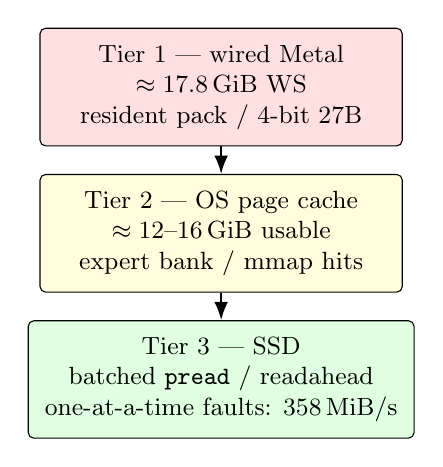
\begin{tikzpicture}[
  font=\small,
  box/.style={draw,rounded corners=2pt,align=center,inner sep=6pt,minimum width=4.6cm},
]
\node[box,fill=red!12] (t1) {Tier 1 --- wired Metal\\$\approx 17.8$\,GiB WS\\resident pack / 4-bit 27B};
\node[box,fill=yellow!14,below=0.35cm of t1] (t2) {Tier 2 --- OS page cache\\$\approx 12$--16\,GiB usable\\expert bank / mmap hits};
\node[box,fill=green!12,below=0.35cm of t2] (t3) {Tier 3 --- SSD\\batched \texttt{pread} / readahead\\one-at-a-time faults: 358\,MiB/s};
\draw[-{Latex},thick] (t1) -- (t2);
\draw[-{Latex},thick] (t2) -- (t3);
\end{tikzpicture}
\caption{Three-tier unified memory. Stock mlx-lm and llama.cpp put the whole 19\,GiB 35B bank in tier~1 and fail. \slotbank{} puts $\approx 3.46$\,GiB in tier~1 and lets tiers~2 and~3 serve misses. On dense 27B the same picture is ``fit the 15\,GiB pack in tier~1, then stop inventing wrappers.''}
\label{fig:tiers}
\end{figure}

macOS drives free pages toward zero by design. Admission therefore keys on \emph{reclaimable} pages (free + speculative + inactive + purgeable), not on ``Pages free.'' Shedding the prompt cache on low free pages was a self-inflicted miss after every request.

\subsection{Qwen3.8-27B}

Qwen3.8-27B is a dense causal LM with a vision encoder~\citep{qwen38card}. Language-model facts used by the runtime:

\begin{center}
\begin{tabular}{@{}ll@{}}
\toprule
Quantity & Value \\
\midrule
Parameters & $27.78$B \\
Layers / pattern & 64, $16\times(3\times\mathrm{GDN}{+}\mathrm{FFN},\ 1\times\mathrm{Attn}{+}\mathrm{FFN})$ \\
Hidden / FFN & $5120$ / $17408$ \\
Vocab (untied) & $248320$ \\
GDN heads $(QK, V)$, $d$ & $(16, 48)$, $128$ \\
Full attn heads $(Q, KV)$, $d$ & $(24, 4)$, $256$ \\
Full-attn KV & $\approx 64$\,KiB/token \\
GDN state & $O(1)$, $\approx 150$\,MiB, \texttt{float32} \\
Context & $262144$ native, YaRN to $1$M~\citep{yarn2024} \\
MTP & trained, sidecar $\approx 66.4$M / $239$\,MB \\
\bottomrule
\end{tabular}
\end{center}

Official sampling~\citep{qwen38card}: thinking $T{=}1.0$, $p{=}0.95$, $k{=}20$; instruct $T{=}0.7$, $p{=}0.80$, $k{=}20$. OMP sends temperature $1.0$. The envelope remaps $T \ge 0.99$ onto that pair. The runtime does not force $T{=}0$ to chase a bench.

Vendor quality numbers (Claude Code harness, $T{=}1.0$) place the model at 61.7 SWE-bench Pro, 90.3 LiveCodeBench v6, 89.2 GPQA Diamond, 84.3 OSWorld-Verified---ahead of Qwen3.6-27B on every agent/coding row in the card, and ahead of Opus~4.6 Max on several software-engineering benches. Those are capability scores, not Mac scores. 4-bit is a quality tax; it is still the same 27B.

Packed Metal GDN is eligible: $D_k{=}128$ is divisible by 32 and $D_v$ is divisible by 8.

\begin{figure}[t]
\centering
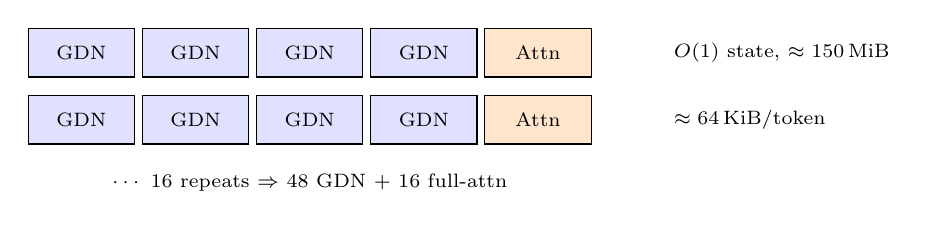
\begin{tikzpicture}[
  font=\scriptsize,
  cell/.style={draw,minimum width=1.35cm,minimum height=0.62cm,align=center},
  gdn/.style={cell,fill=blue!12},
  att/.style={cell,fill=orange!20}
]
\foreach \i in {0,1,2,3} {
  \node[gdn] at (\i*1.45,0) {GDN};
}
\node[att] at (5.8,0) {Attn};
\foreach \i in {0,1,2,3} {
  \node[gdn] at (\i*1.45,-0.85) {GDN};
}
\node[att] at (5.8,-0.85) {Attn};
\node[align=center,font=\scriptsize] at (2.9,-1.65) {$\cdots$ 16 repeats $\Rightarrow$ 48 GDN + 16 full-attn};
\node[align=left,font=\scriptsize,anchor=west] at (7.4,0) {$O(1)$ state, $\approx 150$\,MiB};
\node[align=left,font=\scriptsize,anchor=west] at (7.4,-0.85) {$\approx 64$\,KiB/token};
\end{tikzpicture}
\caption{Qwen3.8-27B hybrid block. The 3{:}1 pattern is why \texttt{can\_trim\_prompt\_cache} is false: most layers store a recurrent summary, not a per-token tensor that PagedAttention can slice.}
\label{fig:hybrid}
\end{figure}

A Gated DeltaNet layer maintains a matrix-valued state $S_t$ updated by a gated delta rule~\citep{yang2024gateddelta}:
\begin{equation}
  S_t \;=\; S_{t-1}\bigl(I - \beta_t k_t k_t^\top\bigr) + \beta_t v_t k_t^\top,
\end{equation}
with an additional input-dependent gate on the decay. The state after token $t$ is a function of the entire prefix $x_{1:t}$. There is no implemented right-inverse that would let a runtime drop the last $k$ tokens and recover $S_{t-k}$ from $S_t$ alone. That is the mathematical content of ``untrimmable.'' Full-attention layers beside it \emph{are} trimmable KV tensors; \texttt{can\_trim\_prompt\_cache} is a conjunction over the whole stack and therefore false.

\subsection{Speculative decoding as an acceptance lottery}

Let $q$ be the drafter, $p$ the target, and $K$ the trained block. Leviathan--Chen acceptance of draft token $i$ is
\begin{equation}
  \alpha_i \;=\; \min\bigl(1,\; p(x_i\mid x_{<i})/q(x_i\mid x_{<i})\bigr).
\end{equation}
Expected accepted length on a well calibrated student is bounded by $K$. Forcing $K{=}5$ on a head trained at 3, or leaving $K{=}1$ after a low-accept think dump, is not a tuning knob. The algorithm has changed. Expected tok/s under exact verify is
\begin{equation}
  \tau_{\mathrm{spec}} \;\approx\; \frac{\mathbb{E}[1+A]}{T_{\mathrm{draft}}+T_{\mathrm{verify}}},
\end{equation}
where $A$ is accepted extras. On this Air, $T_{\mathrm{verify}}$ is one 15\,GiB target forward ($\approx 175$\,ms greedy). Native MTP at $K{=}3$ measures $2.36\times$ on a high-accept count prompt and $1.74\times$ on code. Perfect always-accept $K{=}3$ is $\approx 17$ tok/s---the in-tree ceiling. DFlash2's longer $K{=}8$ does not beat that ceiling here because the student is heavier ($\approx 1$\,GiB vs.\ 239\,MB) and accept on code is worse.

Cost and correctness come apart here. A cheaper $T{>}1$ backbone verify that flips about 4\% of argmax decisions is not speculative decoding of the 27B. It is another model that happens to share a checkpoint directory.

\subsection{Clocks}

I use four clocks. Mixing them is the usual reason two Mac write-ups cannot be compared.

\begin{definition}[Cold end-to-end]
Tokens divided by wall time from process launch, including load and prefill.
\end{definition}
\begin{definition}[Warm sustained decode]
Tokens after the first token, over the whole run.
\end{definition}
\begin{definition}[Time-to-first-token]
Wall time from request accept to the first emitted token. On this hybrid, TTFT \emph{is} prefill, not MTP.
\end{definition}

A fourth number, compute-only ceiling, appears only when I/O is stubbed out on the MoE path.

\subsection{\texorpdfstring{Why 24\,GB is a different machine from 128\,GB}{Why 24 GB is a different machine from 128 GB}}

Let $B_{\mathrm{Air}}{=}120$\,GB/s and $B_{\mathrm{Max}}{=}400$\,GB/s (M3 Max). Linear scaling of an oMLX Metal baseline of 19.8 decode tok/s and 32.6 MTP tok/s~\citep{omlx2874} predicts $5.94$ and $9.78$ on the Air. The Air measures $5.71$ greedy and $9.95$ MTP (code). Decode is already on the Max curve. ANE prefill of $267$ tok/s scales to a fictional $80$ if bandwidth were the only term; the Air measures $\approx 48$ without ANE. ANE compilation unpacks layers toward fp32 (I have seen $\approx 16$\,GiB spikes quoted) and keeps procedure banks. Peak oMLX footprints at 16K are $70$--$80$\,GB with \texttt{iogpu.wired\_limit\_mb=110000}. There is no leave-free setting that turns a 24\,GB Air into that machine.

%======================================================================
\section{Design Thesis}
\label{sec:thesis}

\begin{proposition}[Fit first, then stock kernels]
If the hot bytes fit the leave-free working set, stock MLX kernels beat any slot or stream wrapper. If they do not, shrink residency (slots, quant, envelope) until they do. Do not invent a slower kernel to save a copy that still does not fit.
\end{proposition}

\begin{proposition}[Untrimmable state is a prefix monoid]
\texttt{ArraysCache} is a running summary $s_t = f(s_{t-1}, x_t)$. The only correct reuse is an exact stored prefix $x_{1:n}$ with $s_n$ restored. A longest-common-prefix that is a \emph{proper} subset of a stored snapshot would require a right-inverse of $f$. None is implemented; \texttt{trim} is a no-op.
\end{proposition}

\begin{proposition}[Speedups that change tokens are not speedups]
Any method whose output distribution is not the 27B at the requested sampler---token dropping, layer skipping, a 4B writer, abliterated weights, KV-quant-with-draft---is out of scope, including as a ``draft'' that the 27B merely checks for style.
\end{proposition}

Most of the implementation is those three rules applied until I ran out of ideas that still obeyed them.

I also refuse unlabelled throughput. Every number below is one of: cold end-to-end from process launch; warm sustained decode after the first token; a compute-only ceiling with I/O stubbed; or time-to-first-token (prefill on this hybrid). If a figure has no clock, that is a mistake in the draft, not a fifth kind of measurement.

\begin{proposition}[Name the clock]
Cold end-to-end, warm sustained decode, compute-only ceiling, and TTFT are the only throughput clocks used in this report.
\end{proposition}

\begin{figure}[t]
\centering
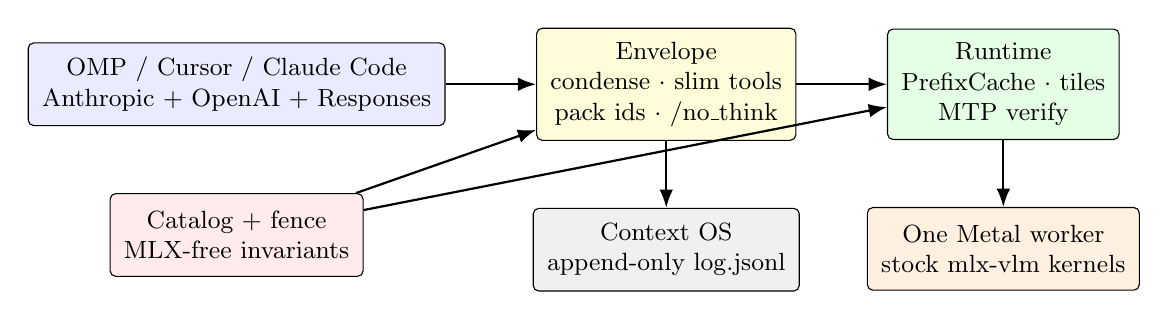
\begin{tikzpicture}[
  font=\small,
  box/.style={draw,rounded corners=2pt,align=center,inner sep=5pt,minimum height=1.05cm},
  arr/.style={-{Latex},thick}
]
\node[box,fill=blue!8] (omp) {OMP / Cursor / Claude Code\\Anthropic + OpenAI + Responses};
\node[box,fill=yellow!15,right=1.15cm of omp] (env) {Envelope\\condense $\cdot$ slim tools\\pack ids $\cdot$ /no\_think};
\node[box,fill=green!10,right=1.15cm of env] (rt) {Runtime\\PrefixCache $\cdot$ tiles\\MTP verify};
\node[box,fill=orange!12,below=0.85cm of rt] (metal) {One Metal worker\\stock mlx-vlm kernels};
\node[box,fill=gray!12,below=0.85cm of env] (os) {Context OS\\append-only log.jsonl};
\node[box,fill=red!8,below=0.85cm of omp] (cat) {Catalog + fence\\MLX-free invariants};
\draw[arr] (omp) -- (env);
\draw[arr] (env) -- (rt);
\draw[arr] (rt) -- (metal);
\draw[arr] (env) -- (os);
\draw[arr] (cat) -- (env);
\draw[arr] (cat) -- (rt);
\end{tikzpicture}
\caption{Request path. OMP still owns the harness. Metal sees a condensed, cache-stable projection. MLX imports are confined to three files.}
\label{fig:arch}
\end{figure}

%======================================================================
\section{Method I: Expert-Slot Cache for MoE}
\label{sec:moe}

\subsection{Steal, remap, fill, freeze}

A Switch-linear stores experts stacked as $(E, d_{\mathrm{out}}, d_{\mathrm{in}})$. Stock MLX \texttt{gather\_qmm} indexes that stack. If $E{=}256$ and the stack is 16.9\,GiB, the gather touches memory the Air does not have. \slotbank{}:

\begin{enumerate}[leftmargin=1.4em]
\item Steals the stacked tensors off every \texttt{SwitchLinear} / \texttt{QuantizedSwitchLinear} so the stock gather cannot see them.
\item Remaps router ids $\to$ slot ids on Metal. Decode does not \texttt{.tolist()} the router.
\item Fills only misses into a $C$-slot pack, in place, with batched readahead.
\item Sizes $C$ once at load and freezes it for a generate. It does not softmax live RAM every token.
\end{enumerate}

\texttt{install\_expert\_slots} is a no-op ($0$) on dense modules, which is how the 27B shares the process. Wrapping keys off class \emph{name}, so the same code attaches to \texttt{mlx-lm} and \texttt{mlx-vlm} Switch types. Architectures that exist only in \texttt{mlx-vlm} (\texttt{deepseek\_v4}, \texttt{kimi\_k3}, \texttt{minimax\_m3}, experimental \texttt{qwen4\_exp}) take that loader first.

\subsection{Why a larger pack was slower}

Default $C{=}16$ is $2\times$ top-8. On 35B-A3B the measured interior optimum is $C{=}32$ (3.46\,GiB wired). $C{=}64$ (5.57\,GiB) takes 31\% fewer misses and still reads about twice as many bytes from disk, because the extra 2.1\,GiB came out of the page cache that was serving those misses. Routing is skewed: top-32 experts carry 53.7\% of traffic, top-64 carry 76.2\%. Doubling $C$ from 32 to 64 buys 22 points of hit rate and loses linear cache. On a machine where 16.9\,GiB of experts fits in cache outright, the trade reverses. On this laptop it does not.

Page-cache state dominates A/B order. Running $C{=}32$ then $C{=}64$ makes $C{=}64$ look $1.9\times$ faster because the first run warmed the cache. Only alternating repeats are reported.

\subsection{Decode vs.\ prefill eligibility}

A forward is eligible for the slot path if every routed id can be resident at once: $T{=}1$, or a short speculative verify with $n_{\mathrm{ids}} \le C$. Larger passes take a prefill path that does not evict an expert the gather still needs. That bound is correctness, not a speed knob.

\subsection{When not to use slots}

OLMoE-1B-7B 4-bit (3.6\,GB) fits. Stock \texttt{mlx-lm} is $53$--$56$ tok/s at 3.66\,GiB. Slots at $C{=}16$ are $14$--$19$ tok/s at 1.13\,GiB. That is a bad deal. The README states it as a rule: use stock when the bank fits.

\subsection{Capacity sweep}

Re-measured after the read-path work, 35B-A3B, cold start to 256 tokens:

\begin{table}[ht]
\centering
\caption{35B-A3B capacity sweep on this Air after the read-path work. $C{=}32$ is the interior maximum.}
\label{tab:csweep}
\begin{tabular}{@{}rrll@{}}
\toprule
$C$ & Active & Cold end-to-end (2 reps) & Warm decode \\
\midrule
8 & 1.88\,GiB & 3.32 / 4.19 & 4.54 / 5.78 \\
16 & 2.41\,GiB & 4.06 / 4.30 & 5.62 / 6.02 \\
\textbf{32} & \textbf{3.46\,GiB} & \textbf{4.10 / 4.88} & \textbf{5.97 / 7.15} \\
48 & 4.52\,GiB & 3.55 / 4.57 & 5.20 / 6.80 \\
64 & 5.57\,GiB & 3.36 / 3.78 & 4.84 / 5.27 \\
96 & 7.68\,GiB & 3.32 & 4.82 \\
\bottomrule
\end{tabular}
\end{table}

Direct evidence that extra slots steal the cache that serves misses, alternating $C{=}32$ and $C{=}64$ three times against a fully warm cache:

\begin{table}[ht]
\centering
\caption{Alternating $C{=}32$ vs.\ $C{=}64$ against a warm page cache. Miss rate falls; disk traffic rises.}
\label{tab:c3264}
\begin{tabular}{@{}llll@{}}
\toprule
$C$ & tok/s & Miss/call & Disk read per token (MiB) \\
\midrule
32 & 8.60 / 8.74 / 8.53 & 3.012 & 17.1 / 15.5 / 22.0 \\
64 & 7.35 / 6.31 / 5.93 & 2.089 & 24.2 / 39.0 / 41.5 \\
\bottomrule
\end{tabular}
\end{table}

$C{=}64$ takes 31\% fewer misses and still reads about twice as much from disk, because its extra 2.1\,GiB of pack came out of the page cache serving the misses it still takes. Routing concentration explains the diminishing hit-rate: top-32 experts carry 53.7\% of traffic, top-64 carry 76.2\%. Doubling $C$ from 32 to 64 buys 22 points of hit rate and loses linear cache.

\subsection{I/O path evolution}

Cold 35B decode was 73\% file read + pack write. Three changes moved the needle (Table~\ref{tab:iowins}).

\begin{table}[ht]
\centering
\caption{35B-A3B at $C{=}64$, decode, after each I/O change.}
\label{tab:iowins}
\begin{tabular}{@{}lrr@{}}
\toprule
Change & Cold tok/s & Warm tok/s \\
\midrule
Private-queue \texttt{DeviceCopy}, one wait/layer & 1.16 & 5.93 \\
In-place slice fill, no pack eval in \texttt{copy\_missing} & 2.50 & 2.89 \\
mmap + batched \texttt{MADV\_WILLNEED} & 7.66 & 8.22 \\
\bottomrule
\end{tabular}
\end{table}

The first change removed $\approx 16$ cross-queue stalls per token ($\approx 3.5$\,ms each, moving 1.4\,MiB---about $300\times$ the time those bytes deserve). Cold start improved $6.7\times$ and the cold/warm gap closed. Prefill of an 865-token prompt moved $126.4\,\mathrm{s}\to 49.4\,\mathrm{s}$ with batched readahead, $\approx 43$\,s once \texttt{sorted\_indices} was threaded through, and $37.3$\,s with optional waves (\texttt{SLOTBANK\_WAVES=1}). Waves split one gather, which changes float16 split-K rounding ($\approx 1$\,ULP/layer, $\approx 4\%$ relative on final logits). Greedy tokens matched $48/48$ when measured, but bit-identical is the accuracy contract, so waves stay off.

\subsection{What this SSD actually prices}

Profiling the miss path by phase, not by stubbing whole stages, found the cost was not where the stage-level numbers implied (35B-A3B, $C{=}32$, 48 tokens):

\begin{table}[ht]
\centering
\caption{Miss-path phase budget. The hint cost $3\times$ the read.}
\label{tab:madvise}
\begin{tabular}{@{}lrr@{}}
\toprule
Phase & ms/token & Share \\
\midrule
\texttt{madvise(MADV\_WILLNEED)} prefetch & 179.9 & 45.9\% \\
\texttt{mx.eval} + \texttt{meta[0].item()} sync ($40\times$) & 124.2 & 31.7\% \\
Read I/O & 54.6 & 13.9\% \\
Scatter into pack & 1.5 & 0.4\% \\
Attention + GEMM + sampler & 31.6 & 8.1\% \\
\bottomrule
\end{tabular}
\end{table}

The reads themselves match what this SSD should deliver. The \emph{hint} costs three times the read it hints, because \texttt{MADV\_WILLNEED} is per-page VM bookkeeping: a layer advises 27 rows $\times$ 32 pages, $\approx 34{,}500$ pages per token. Deleting the advise is not an option---it is worth $2\times$ on its own ($2.43\to 1.20$ tok/s)---because without it mmap faults are taken one at a time.

Uncached (\texttt{F\_NOCACHE}) reads show what the device wants: request size and queue depth, not locality. Random and sequential differ by ${<}10\%$ above 64\,KiB. Expert rows are 512\,KiB (weights) and 32\,KiB (scales/biases), nine reads per expert. Since \texttt{pread} releases the GIL and does no VM work, the fix is to take the pread path \emph{and skip the advise}. \texttt{SLOTBANK\_READ\_THREADS} defaults to 8. A 400-token greedy A/B (identical \texttt{miss/call} to three decimals) measured 5.2 vs.\ 3.3 sustained tok/s ($1.58\times$), bit-identical 40/40.

\subsection{Reading straight into the pack}

A miss used to travel \texttt{pread} $\to$ \texttt{bytes} $\to$ \texttt{mx.array} $\to$ \texttt{.view()} $\to$ \texttt{.reshape()} $\to$ \texttt{pack[slot]=row}. The bytes on disk are already in the pack's layout. That chain was $\approx 218$\,MiB/token of transient host copies and $\approx 1137$ MLX graph nodes. \texttt{os.preadv} writes into \texttt{memoryview(pack)} instead. Seven paired 120-token warm runs: mean $5.820\to 7.376$ tok/s ($1.27\times$; median ratio $1.31\times$). Output is bit-identical to the independent mmap path (100/100 ids), 3771 preadv calls with zero fallbacks. Guarded by \texttt{test\_preadv\_lands\_rows\_in\_pack\_slots}.

After this change the warm budget at 6.68 tok/s (149.7\,ms/token) is 56.3\% GPU sync ($40\times$), 35.8\% preadv, 8.0\% attention/GEMM/gather. Scatter is gone. Overlapping host and GPU work is the obvious next move. Measured with \texttt{mx.async\_eval} on balanced layer-sized work: 24\% overlap efficiency. Against the $\approx 18$\,ms of \texttt{down\_proj} reads that are eligible, that is $\approx 4$\,ms---2.7\%---for a change that would split \texttt{copy\_missing} by bank group. I left the overlap unimplemented.

\subsection{The sync that was a Python idiom}

\texttt{mx.eval} makes an array host-readable. Reading a scalar afterwards with \texttt{meta[0].item()} does \emph{not} read that host memory: it builds a fresh lazy slice on the Metal stream and blocks on a second command buffer. On an already-evaluated array: \texttt{.item()} is $224.7\,\mu\mathrm{s}$; \texttt{memoryview} is $0.8\,\mu\mathrm{s}$; \texttt{.tolist()} is $0.6\,\mu\mathrm{s}$. The copy path ran this once per MoE layer: $40\times 224\,\mu\mathrm{s}$ of avoidable command-buffer latency per token, hiding inside ``GPU sync.'' Reading through the buffer protocol: mean $+6.9\%$ tok/s, 10.9\,ms saved vs.\ 9.0\,ms predicted, bit-identical 100/100. The general lesson is worth more than the 6.9\%: \texttt{.item()} after \texttt{eval} is a GPU round trip, not a host read. Any \texttt{.item()} on a per-layer path is a latency bug.

A full attribution of the $\approx 167$\,ms token budget puts the CPython interpreter proper at 3--5\,ms, or 2--3\% (Table~\ref{tab:python}). Rewriting the decode loop in C++/Rust is projected at 6--9\%---it deletes essentially all Python and touches none of the compute, device I/O, or driver latency---for a large rewrite, and it would drop mlx-lm compatibility and the bit-identical contract. I did not do it. The \texttt{memoryview} change recovered more than that projected 6--9\% by itself.

\begin{table}[ht]
\centering
\caption{Approximate per-token budget on 35B-A3B after the preadv and \texttt{memoryview} changes.}
\label{tab:python}
\begin{tabular}{@{}lrl@{}}
\toprule
Term & ms/token & What it is \\
\midrule
GPU compute & $\sim 50$ & Metal (matches 19--21 tok/s stubbed ceiling) \\
Device I/O, depth 8 & $\sim 46$--48 & kernel + SSD \\
Host memcpy + Metal alloc & $\sim 14$ & libc / MLX allocator \\
Command-buffer stall & $\sim 15$--25 & driver \\
Redundant \texttt{.item()} (fixed) & $\sim 7$--11 & Metal, caused by a Python idiom \\
\texttt{ThreadPoolExecutor} & $\sim 7$ & Python \\
MLX graph construction & $\sim 5$--8 & MLX C++, called from Python \\
CPython bytecode & $\sim 3$--5 & Python \\
\bottomrule
\end{tabular}
\end{table}

What actually caps the MoE path is structural: the per-layer sequence GPU-ensure $\to$ host-sync $\to$ device-read $\to$ host-scatter $\to$ GPU-gather is fully serialised 40 times per token. Layer $L$'s expert set is unknown until layer $L{-}1$ has run. Overlapping those phases is worth up to $\approx 45$\,ms/token and is blocked by that data dependence, not by the language.

\subsection{Context scaling on the MoE path}

At $C{=}32$, decode throughput is flat in context. The cost of long context is prefill, in time and in peak memory (Table~\ref{tab:ctxscale}). Active memory barely moves because only 10 of 40 layers are full-attention; the other 30 are GDN with constant-size state. KV is $\approx 20$\,KiB/token, so 128k is $\approx 2.5$\,GiB. KV is not the constraint. The prefill peak is: extrapolating, $\approx 16$\,GiB around 32k, which is where it meets the working set.

\begin{table}[ht]
\centering
\caption{35B-A3B, $C{=}32$. Decode is flat; prefill and peak grow.}
\label{tab:ctxscale}
\begin{tabular}{@{}rrrrrr@{}}
\toprule
ctx & Prefill & tok/s & Miss/call & Active & Peak \\
\midrule
128 & 19.6\,s & 1.99 & 4.079/8 & 3.459\,GiB & 5.567\,GiB \\
512 & 28.4\,s & 2.42 & 3.490/8 & 3.469\,GiB & 6.053\,GiB \\
2048 & 57.5\,s & 2.13 & 3.635/8 & 3.498\,GiB & 7.134\,GiB \\
4096 & 105.6\,s & 1.82 & 2.700/8 & 3.537\,GiB & 9.310\,GiB \\
\bottomrule
\end{tabular}
\end{table}

\subsection{Compute-only ceiling}

Stubbing the copy path at default $C{=}32$, eight repeats: median 19.23 tok/s (min 18.40, max 21.25). From 7.96 warm there is roughly $2.4\times$ of headroom left, all of it in I/O shape. An earlier single run at $C{=}64$ reported 33.4; two other runs of the same measurement gave 21.0 and 20.1, so 33 is treated as an outlier. The remaining gap cannot be pushed past the ceiling without attacking the attention/GEMM stack, which is MLX's domain.

\subsection{\texorpdfstring{T${>}1$ numerics are not a copy-path bug}{T>1 numerics are not a copy-path bug}}

Building MTP \emph{inside} the slot runtime would mean verifying $[\mathrm{confirmed},\mathrm{drafted}]$ in one $T{=}2$ backbone pass. On this hybrid that pass does not compute the same logits as two $T{=}1$ passes. Measured on Qwen3.5-4B through mlx-lm:
\[
\max|\Delta\mathrm{logit}|_{T=1\text{ vs }T=2}=1.562\times 10^{-1},\qquad
\mathrm{mean}|\Delta\mathrm{logit}|=2.563\times 10^{-2}.
\]
The chunked scan used for $T{>}1$ in Gated DeltaNet differs from the recurrent step used at $T{=}1$. On the 35B this flips $\approx 4\%$ of argmax decisions. A drafter head plus perfect state rollback would still yield a different model. mlx-vlm's specialised path is byte-identical (273 bytes exact at draft blocks 2 and 4 on the same 4B) because it verifies per token with GEMV kernels (\texttt{qwen3\_5\_target\_verify\_gemv} and friends) rather than a batched GEMM, plus \texttt{rollback\_speculative\_cache}. The accuracy-preserving path is therefore to run under mlx-vlm's model classes, not to reimplement those kernels. That is already compatible: wrapping keys off class \emph{name}.

The economic statement is separate. At 94.3\% copy the verify pass could not pay for itself at any acceptance rate; after the I/O work, at 43.3\% copy, it projects $\approx 1.19\times$ on the MoE path. Dense 27B already has a matching sidecar and is past that test.

%======================================================================
\section{Method II: Dense 27B Fit Path}
\label{sec:dense}

Dense 27B has no $C$. The slotbank move is the same sentence: shrink hot bytes until stock kernels fit.

\paragraph{Quant.} Daily pack is affine 4-bit, $\approx 15$\,GiB. Mixed 3.5\,bpw is the quality pack and measures $0.94$--$1.11$ tok/s on this Air (kernel ceiling of 3-bit overrides, not a wrapper tax). Uniform 3-bit loses MMLU-Pro (54.2 vs.\ 61.0). Unquantized bf16 is rejected.

\paragraph{Leave-free.} Default leave-free on 24\,GB is 8\,GiB (16\,GiB WS). 15\,GiB + MTP does not fit. \texttt{--leave-free 6g} (18\,GiB WS) is required. Admission uses \texttt{stored + KV $\le$ total $-$ leave\_free} before load.

\paragraph{Vision.} The tower is $\approx 0.4$\,GiB. Text-only load through \texttt{mlx-lm} drops it. Daily serve keeps \texttt{--vision}. Omitting vision does not remove the 30\,s pin.

\paragraph{Pin vs.\ ready.} \texttt{Engine} mmaps and builds graphs on the Metal worker, sets \texttt{\_ready} for OMP \texttt{/models/load}, then \texttt{pin()}s the 15\,GiB pack. The picker spinner can return before pin. First generate still waits. Restarting serve re-pays it. Keep the process up.

\paragraph{Allocator.} A 512\,MiB MLX free-cache forces Metal malloc per layer during a large tile~\citep{mlx3350}. Prefill raises the pool to 2\,GiB, then restores 512 so idle activations do not sit at peak.

\paragraph{Not built.} No \texttt{layer\_slots.py}. Streaming GDN from SSD is the 1 tok/s path. No ANE: MLX 0.32.1 exposes Metal GPU, and a second fp16 compile spike does not sit beside 15\,GiB on 24\,GB.

%======================================================================
\section{Method III: Hybrid-Safe Speculation}
\label{sec:spec}

\subsection{The silent bug}

\begin{algorithm}[t]
\caption{Unsafe rewind (mlx-lm class)}
\begin{algorithmic}[1]
\State \textbf{on reject:} \texttt{trim\_prompt\_cache}(target, $n_{\mathrm{draft}}-n_{\mathrm{accept}}$)
\If{\textbf{not} \texttt{can\_trim\_prompt\_cache}}
  \State \Return $0$ \Comment{no-op; state of rejected drafts remains}
\EndIf
\end{algorithmic}
\end{algorithm}

Qwen3.5-35B-A3B builds 30 \texttt{ArraysCache} + 10 \texttt{KVCache}; \texttt{can\_trim} is false. \slotbank{} refuses that path. Prompt-lookup speculation is compiled and gated on \texttt{\_can\_speculate}, which is false here.

\subsection{The safe path}

Daily 27B uses \texttt{mlx-vlm}'s \texttt{generate\_step} with \texttt{draft\_model}, \texttt{draft\_kind=mtp}, trained block size 3, and a \texttt{prompt\_cache} already filled by runtime tiles. Rollback is \texttt{rollback\_speculative\_cache}. KV bits are forced off when a draft is set. The sidecar is not a second LM: 66.4M parameters, trained $K{=}3$. DFlash2 ($K{=}8$, $\approx 1$\,GiB) remains valid and lost the A/B on this Air (11.76 / 9.10 vs.\ 13.47 / 9.95). Two drafters in one generate are rejected: one \texttt{draft\_model}, one verify.

\subsection{\texorpdfstring{Trained $K$ every request}{Trained K every request}}

A previous DAIS policy shrank $K$ after low accept and left it there. The next OMP ``hi'' ran at $K{=}1$ (greedy speed). \texttt{\_arm\_draft\_block} resets to the trained cap at the start of every \texttt{\_iter\_draft}. Growing past trained $K$ is how MTP block 6 measured $0.85\times$ on 4B.

\begin{algorithm}[t]
\caption{\texttt{\_arm\_draft\_block}: persist is not a speedup}
\begin{algorithmic}[1]
\If{draft cap is set}
  \State $K \leftarrow K_{\mathrm{trained}}$ \Comment{3 for MTP, 8 for DFlash2}
\EndIf
\end{algorithmic}
\end{algorithm}

\subsection{Last token only}

After pyramid prefill, \texttt{generate\_step} receives a $1$-token tensor: the last prompt id. Older \texttt{mlx-vlm} disabled chunked prefill when a drafter was set. The runtime owns tiles so that disable does not re-prefill $N$. mRoPE is not primed on the full prompt before decode: the helper wrote deltas the step then nulled, which on an 8k envelope was a full-prompt rope index and a discard.

\subsection{Session integrity}

If DFlash accepted tokens past EOS, attention \texttt{offset} can run ahead of recorded ids. \texttt{dflash\_session\_ok} requires every attention-layer offset equal $|\mathrm{fed}|$, else the cache is dropped. Reusing a long cache would condition the next turn on tokens the client never saw.

\subsection{Why mlx-lm speculation is banned, in full}

The bug is not theoretical. \texttt{speculative\_generate\_step} rewinds by calling \texttt{trim\_prompt\_cache} and ignores both \texttt{can\_trim\_prompt\_cache} and the return value~\citep{slotbankrepo}. On Qwen3.5-35B-A3B the cache is $30\times$ \texttt{ArraysCache} + $10\times$ \texttt{KVCache}; trim returns 0; rejected drafts remain in the recurrent summary; every subsequent token is conditioned on tokens that are not in the output. There is no exception and no warning. A second silent path: Qwen3 vocab 151936 and Qwen3.5/3.8 vocab 248320 are not interchangeable. A 4B drafter that ``shares the family name'' fails both width ($\approx 2560$ vs.\ $5120$) and that vocab trap.

The suggested upstream fix is fail-fast. The local fix is stronger: the daily door never calls that function. Prompt-lookup $n$-gram drafting is compiled and gated on \texttt{\_can\_speculate}, which is false here, so it cannot become an accidental second drafter.

%======================================================================
\section{Method IV: Exact-Prefix Cache}
\label{sec:prefix}

\subsection{Reuse relation}

\begin{definition}[Live append]
Given fed ids $f$ and new ids $x$, reuse $|f|$ iff $f$ is a proper prefix of $x$ and $|x|>1$. Otherwise reuse is $0$ and $x$ is prefills in full.
\end{definition}

OMP re-encodes the whole chat every turn, so $f$ (prompt + generated) is almost never a prefix of $x$. The system head can be. \texttt{draft\_reuse} tries live append first, then the longest exact stored snapshot with length in $[32, |x|)$.

\begin{algorithm}[t]
\caption{Exact-prefix reuse (never a partial trim)}
\begin{algorithmic}[1]
\State $(r, \mathrm{feed}) \leftarrow \mathrm{draft\_feed}(f, x, \mathrm{hasCache})$
\If{$r > 0$} \Return $(r, \mathrm{feed})$
\EndIf
\If{stored prefix $p$ exists $\wedge$ $|p|\ge 32$ $\wedge$ $p = x_{1:|p|}$}
  \State restore $s_{|p|}$ into a \emph{new} cache
  \State \Return $(|p|, x_{|p|+1:})$
\EndIf
\State \Return $(0, x)$
\end{algorithmic}
\end{algorithm}

The live cache is not trimmed to $p$. It may hold extra tokens. Restore writes into a fresh cache.

\subsection{Qwen template is not a prefix}

Three encodings are not prefixes of the next OMP turn~\citep{qwen31826,mlxengine176}:

\begin{enumerate}[leftmargin=1.4em]
\item \texttt{add\_generation\_prompt} injects empty think tags when thinking is off. Historical assistant turns omit them.
\item Envelope \texttt{/no\_think} is last-ask only. History omits that suffix.
\item A last-user-only condense rewrites user-1 when it becomes history.
\end{enumerate}

\texttt{PromptIds.stable\_prefix\_n} is the common prefix of the full encode and the same messages without the generation prompt and without \texttt{/no\_think}. Snap points keep that index on short prompts and $2048$ on long ones. A hardcoded 128 used to split every short ``hi'' into two 27B forwards. Geometric 256/512/1024 crumbs split the first 2k of an 8k envelope; eviction already dropped them first.

LM Studio's template fix reports $4.96\,\mathrm{s} \to 0.20\,\mathrm{s}$ ($25\times$) on follow-up TTFT. This runtime does not patch Jinja; it snaps at the body.

\subsection{Snapshot budget}

A 10k envelope copy was $\approx 790$\,MiB extra RAM and jetsamed 24\,GB. \texttt{MAX\_SNAP}${}=2048$, default 384\,MiB. Eviction drops the shortest snapshot first so a system head outlives crumbs. \texttt{put} refuses oversize and duplicate keys.

\subsection{Restore must write offset}

\texttt{KVCache.state}'s setter is supposed to set \texttt{offset} from \texttt{keys.shape[2]}. Setters that only write keys/values leave offset at 0~\citep{mlxlm1162}. The suffix would then append onto an empty-looking cache. \texttt{PrefixCache.restore} writes offset from the key length. Rotating caches with \texttt{\_idx} are left alone.

\subsection{Tiles}

Prefill is a loop of \texttt{async\_eval} tiles, one \texttt{mx.eval} at snap points, and \texttt{clear\_cache} once at the end~\citep{mlxvlm945}. Per-chunk eval+clear was the server-vs-vMLX TTFT gap on the same Mac. LM Studio reports $1.5\times$ from chunk $512\to 8192$. \texttt{mlx-swift-lm} reports $9$--$14\times$ from asyncEval on M5 Max and only $1.15$--$1.3\times$ on an M2 Mini: the Air is Mini-class if compute-bound. An 819-token cold prompt is one tile; pipelining cannot overlap a single launch. Tiles pass \texttt{skip\_logits=True} so the 248k \texttt{lm\_head} is not built (Gemma-3 reports $2.6\times$ when that head was actually evaluated).

%======================================================================
\section{Method V: Agent Envelope}
\label{sec:envelope}

OMP's tool catalog alone exceeds 16k tokens. A cwd dump of $\approx 26$k or a \texttt{/tmp $\hookrightarrow$ child-repo} dump of $\approx 39$k produced HTTP 400 or jetsam. The cloud subscription still needs the harness. The Air does not.

\subsection{What is local}

\begin{enumerate}[leftmargin=1.4em]
\item \texttt{condense\_harness\_messages}: system clipped to 256 tokens every turn (was 15\% of 8192 $\approx 1228$, $\approx 25$\,s of cold prefill at 48 tok/s). User dumps use one recipe as last ask or as history. Tool results keep citations or become \texttt{[tool result omitted]}.
\item \texttt{slim\_tools}: names + one-line descriptions, empty JSON schemas, 256-token budget.
\item \texttt{keep\_token\_ids}: sink 25\% (snapped to 512, 1024, 2048), tail 50\%, pyramidal middle. Applied to ids, not to GDN.
\item Hard cap 8192 after pack. \texttt{--no-envelope} restores the refuse.
\item \texttt{/no\_think} on the last ask; \texttt{/think} to reason. Stream holdback strips \texttt{<think>} and \texttt{<|im\_end|>} so OMP does not print analysis as the answer~\citep{qwen38card}.
\item \texttt{--direct} is a stable system prefix, not weight abliteration.
\end{enumerate}

\subsection{What is not local}

OMP YAML is not rewritten for tok/s. Context window advertised to OMP is 65536 so compaction does not loop on a 39k dump; Metal still prefills $\le 8192$. Lying in \texttt{prompt\_tokens} does not shrink OMP's bar. \texttt{omp.py} does not import MLX.

\subsection{Cache-key hygiene}

Serve sets \texttt{CONTEXT\_DIR} so oversized dumps can be logged. It does not compile that log back into the system prefix unless \texttt{SLOTBANK\_CONTEXT\_INJECT=1}. Newest-first compile changes every turn and was the dump the condense just removed---a guaranteed PrefixCache miss.

%======================================================================
\section{Method VI: Context OS}
\label{sec:context}

History longer than the window is kept as an append-only \texttt{log.jsonl}, not as a 1M-token KV tensor. \texttt{compile} selects newest \emph{verbatim} spans that fit a budget (default 4096 tokens) and expands \texttt{file:path:lo-hi} pointers only when the whole span fits \texttt{SLOTBANK\_CONTEXT\_EXPAND} (default 1024). Oversized files stay as citations. The working set is excerpts plus pointers, never an abstractive summary as the only copy. Optional \texttt{SLOTBANK\_CONTEXT\_COMPILER\_URL} must return \texttt{\{working\_set\}}; offline falls back to local extract. One directory per local issue so tasks do not share a cache key. Reordering excerpts is a new prefill.

I think of it as a write-ahead log. Selection into the prompt is lossy; bytes that stay on disk are not rewritten.

\begin{algorithm}[ht]
\caption{Context OS compile (verbatim spans, not a summary)}
\begin{algorithmic}[1]
\State $L \leftarrow$ append-only \texttt{log.jsonl} (newest last)
\State $W \leftarrow [\,]$; $b \leftarrow 0$
\For{record $r$ in reverse($L$)}
  \State expand \texttt{file:path:lo-hi} only if the whole span fits \texttt{EXPAND}
  \If{$b + |r| \le \mathrm{BUDGET}$}
    \State prepend $r$ to $W$; $b \leftarrow b + |r|$
  \Else
    \State keep $r$ as a citation pointer only
  \EndIf
\EndFor
\State \Return $W$ \Comment{never an abstractive rewrite of $L$}
\end{algorithmic}
\end{algorithm}

Serve injects $W$ as a system prefix only when \texttt{SLOTBANK\_CONTEXT\_INJECT=1}. The envelope sets \texttt{CONTEXT\_DIR} so oversized OMP dumps can be logged; it does not compile that log back into the prefix. Newest-first compile changes every turn and is the dump the condense just removed---a guaranteed PrefixCache miss. \texttt{SLOTBANK\_CONTEXT\_EXPAND=0} is citations only (smallest context-stage RAM). Reordering excerpts is a new prefill, not a trim. One directory per local issue so tasks do not share a cache key.

%======================================================================
\section{Method VII: Catalog as Invariants}
\label{sec:catalog}

\texttt{src/slotbank/tps.py} is not documentation. \texttt{catalog\_sound()} is a unit test. It fails if a banned id is marked adopted, if an adopted route sets \texttt{needs\_trim\_cache} or \texttt{changes\_target\_weights}, if daily draft is not sidecar MTP, if the 4-bit pack-read ceiling drifts out of $[7,9]$, or if MTP no longer beats DFlash and $\approx 2\times$ greedy.

Statuses: adopted, attempted, in\_tree, deferred, rejected. Banned-from-adopted includes unquantized bf16, MTP+DFlash, sliding-window KV, hybrid KV paging, named-KV survey, KV-quant-with-draft, PFlash, reverse-spec 4B writer, forced $K{=}5$, layer-stream GDN, async Metal queues, skip-full-attn-on-draft, extra 3-bit, harness-for-tps, 4B-as-27B-drafter, SpecPrefill, CUDA-chunked GDN, DistServe P/D, ANE prefill, and the 2026 Mac ${+}200\%$ headline as a lever.

The catalog is how the project remembers \emph{why} a technique is absent. Without it, the next speed request re-opens ANE, 4B, and paging.

%======================================================================
\section{Implementation}
\label{sec:impl}

\subsection{Process shape}

One process. Inference is MLX; no PyTorch. \texttt{Engine} owns a worker thread because MLX arrays bind to the creating thread. Load and teardown (\texttt{mx.clear\_cache}) run there. Caller-thread close on Python 3.13 fatal-aborted in \texttt{PyThreadState\_Get}.

APIs: OpenAI Chat Completions (Cursor), Anthropic Messages (Claude Code), OpenAI Responses (Codex), plus llama.cpp-shaped \texttt{/models} for OMP discovery. \texttt{slotbank omp} writes static \texttt{llama.cpp} / \texttt{lm-studio} rows into \texttt{\~/.omp/agent/models.yml} without loading weights.

\subsection{Fence}

\begin{center}
\begin{tabular}{@{}ll@{}}
\toprule
May import MLX & Must not \\
\midrule
\texttt{runtime.py} & \texttt{admit.py}, \texttt{omp.py} \\
\texttt{expert\_slots.py} & \texttt{context\_os.py}, \texttt{tps.py} \\
\texttt{offload\_cache.py} & \texttt{prompt.py}, \texttt{decode.py}, API \\
\bottomrule
\end{tabular}
\end{center}

\texttt{tests/test\_fence.py} walks the AST. Package import must not load \texttt{mlx}. That is why this report's catalog can be tested on a Linux VM with no 27B weights. \texttt{decode.py} may import \texttt{os} (stream holdback, env flags) and must not import MLX; that is a fence test, not a style preference. The three MLX files are the only place a Metal array is allowed to exist. Everything else---admit arithmetic, OMP YAML, the context log, the strategy catalog, the envelope---is ordinary Python so a CI runner without weights can still refuse a bad idea.

\subsection{Loader order}

\texttt{SLOTBANK\_LOADER} pins. Else: draft $\Rightarrow$ \texttt{mlx\_vlm} only (rollback lives there); VLM-only types or \texttt{--vision} $\Rightarrow$ vlm first; else \texttt{mlx\_lm} then vlm. \texttt{mlx-vlm} returns a processor; \texttt{encode} lives on \texttt{.tokenizer}. Using the processor as a tokenizer 500'd the first VLM chat.

\subsection{Sampling and stream}

\texttt{SpecialHoldback} is a streaming filter for Qwen stop tags and think blocks. \texttt{finish\_text} splits content / reasoning / tool calls. Tool markup is parsed, not left in the pane. Display name is \texttt{Qwen3.8-27B}, not \texttt{\ldots-agent}, unless the tools door is selected.

%======================================================================
\section{Experimental Methodology}
\label{sec:method}

This section records what I measured, on which machine, under which clock, and what I did not retime. I include it because otherwise the tables get cited as if they were a cluster study. Independent and dependent variables for the software campaign are named in \S\ref{sec:verify}; the Air benches keep the clocks below.

\subsection{Host and software}

\begin{table}[ht]
\centering
\caption{Experimental host. Every 27B and 35B number in this report is this machine unless a citation names another.}
\label{tab:host}
\begin{tabular}{@{}ll@{}}
\toprule
Item & Value \\
\midrule
Machine & Fanless Apple MacBook Air, M4 \\
Unified memory & 24\,GB \\
GPU cores (approx.) & 10 \\
Memory bandwidth & 120\,GB/s \\
Page size & 16\,KiB \\
Metal advertised WS & 17.76--17.8\,GiB \\
OS behaviour & Free pages driven toward zero; reclaimable pages used for admit \\
MLX / mlx-lm (MoE benches) & 0.32.1 / 0.31.3 \\
Daily 27B loader & mlx-vlm (\texttt{generate\_step} + rollback) \\
Python env & project \texttt{.venv} via \texttt{uv}; \texttt{PYTHONPATH=src} \\
Inference backend & MLX only; no PyTorch at serve time \\
\bottomrule
\end{tabular}
\end{table}

\subsection{Checkpoints}

\begin{table}[ht]
\centering
\caption{Checkpoints used. Daily serve is the first 27B row plus its MTP sibling.}
\label{tab:ckpts}
\begin{tabular}{@{}llp{6.4cm}@{}}
\toprule
Id & Size & Role \\
\midrule
Qwen3.8-27B-4bit & $\approx 15$\,GiB & Daily dense target, affine-4 group 64 \\
Qwen3.8-27B-MTP-4bit & $\approx 239$\,MB / 66.4M & Native sidecar, trained $K{=}3$ \\
Qwen3.8-27B-DFlash2-4bit & $\approx 1$\,GiB & Attempted student, trained $K{=}8$ \\
Qwen3.8-27B mixed 3.5\,bpw & $\approx 12$--14\,GiB peak & Quality pack; kernel-slow on this Air \\
Qwen3.5-35B-A3B-4bit & 19.02\,GiB (16.9 experts) & MoE existence proof \\
OLMoE-1B-7B-4bit & 3.6\,GB & Negative control: stock wins \\
Qwen3.5-4B-4bit $\pm$ DFlash & $\approx 2.7$--2.9\,GiB & Different-model 30+ tok/s door \\
\bottomrule
\end{tabular}
\end{table}

\subsection{Clocks, again, as a measurement protocol}

\begin{enumerate}[leftmargin=1.4em]
\item \textbf{Cold end-to-end.} Wall from process launch through $N$ emitted tokens. Includes mmap, graph build, pin, and prefill. Reported for MoE because that is what a user waits for.
\item \textbf{Warm sustained decode.} Tokens after the first token, over the whole run---not a 16-token burst that happens to sit in cached experts.
\item \textbf{Compute-only ceiling.} Same decode with the host copy path stubbed. Answers how much headroom is left in I/O versus GEMM.
\item \textbf{TTFT / prefill.} Request accept to first emitted token. On this hybrid, TTFT \emph{is} prefill. Pin ($\approx 30$\,s) is first-request after boot, reported separately.
\item \textbf{Follow-up TTFT.} Same prefix restored from PrefixCache. A different clock from (4). Mixing them is how ``${+}200\%$'' headlines appear.
\end{enumerate}

Page-cache state dominates MoE A/B. Ordered $C{=}32$ then $C{=}64$ makes $C{=}64$ look $1.9\times$ faster. Only alternating repeats are reported. 27B decode ceilings turn thinking and vision off; daily serve turns them on. OMP temperature stays $1.0$; the envelope remaps $T\ge 0.99$ onto Qwen's documented pair. The runtime is never forced to $T{=}0$ to chase a bench.

\subsection{Correctness oracles}

Bit-identity is the accuracy contract on paths that claim stock tokens. Oracles used:

\begin{itemize}[leftmargin=1.4em]
\item MoE slot vs.\ stock mlx-lm: maxabs $0.0$ on default decode; \texttt{preadv} vs.\ mmap 100/100 token ids; \texttt{memoryview} vs.\ \texttt{.item()} 100/100.
\item Dense draft vs.\ greedy target: \texttt{bit\_match=True} on the 4B DFlash control; 27B MTP/DFlash compared on the same \texttt{parse\_iso\_dates} greedy prefix.
\item mlx-vlm specialised MTP: 273 bytes exact at draft blocks 2 and 4 on 4B.
\item Catalog: \texttt{catalog\_sound()} fails CI if a banned id is adopted, if an adopted route sets \texttt{needs\_trim\_cache} or \texttt{changes\_target\_weights}, if daily draft is not sidecar MTP, if the 4-bit pack-read ceiling drifts out of $[7,9]$, or if MTP no longer beats DFlash and $\approx 2\times$ greedy.
\item Fence: \texttt{tests/test\_fence.py} walks the AST; package import must not load \texttt{mlx}.
\end{itemize}

\subsection{Numbers I could not retime while writing}

The cloud workspace that compiled this PDF has no Metal 27B weights. HTTP there is FakeEngine only. All Air numbers are from the author's laptop, pinned in \texttt{src/slotbank/tps.py} as \texttt{M4\_AIR\_24G} and in the README. In-tree questions that remain unmeasured on the Air after the last code change: PrefixCache restore vs.\ remaining GDN/KV positions, \texttt{generate\_step} after \texttt{skip\_logits} tiles with MTP/\texttt{return\_hidden}/vision, and QMM as the compute floor once stalls are gone.

%======================================================================
\section{Verification Campaign}
\label{sec:verify}

This section is the traceability record. A reader who wants to see whether a sentence in the paper is a reproduction, a pin, or a gap should start here, then open \texttt{verification/campaign\_latest.md} in the repository. The campaign that compiled with this PDF is \texttt{20260902T001357Z} (2 September 2026, 00:14 UTC, Linux x86\_64, Python 3.12.3, no Metal 27B).

I ran three pytest invocations on purpose. Collapsing them would hide the optional-dependency failures and make the filtered tree look like the whole suite.

\begin{table}[ht]
\centering
\caption{Campaign \texttt{20260902T001357Z}. Filtered CI is the project's documented skip list (Hugging Face hub, rich TTY, Metal shed/strip). Full-tree failures are those seven tests; they are named in the log, not ignored.}
\label{tab:campaign}
\begin{tabular}{@{}lrrrrr@{}}
\toprule
Run & passed & failed & skipped & deselected & rc \\
\midrule
Paper claims + fence & 29 & 0 & 0 & 0 & 0 \\
Filtered CI tree & 221 & 0 & 23 & 7 & 0 \\
Full tree & 221 & 7 & 23 & 0 & 1 \\
\bottomrule
\end{tabular}
\end{table}

\subsection{What a claim is allowed to mean}

Every numbered claim has a kind. The campaign is not allowed to promote a kind.

\begin{center}
\small
\begin{tabular}{@{}llp{7.4cm}@{}}
\toprule
Kind & Campaign status & Allowed sentence in this paper \\
\midrule
\texttt{verified\_here} & reproduced on this host & ``The test passed on the campaign host.'' \\
\texttt{air\_pinned} & \texttt{pin\_checked} & ``Measured 2026-08-31 on the Air; the pin has not drifted.'' \\
\texttt{cannot\_retime} & \texttt{documented\_gap} & Named; not a result. \\
\bottomrule
\end{tabular}
\end{center}

\texttt{C-quality} (envelope task quality versus the full OMP harness) and \texttt{C-soak} (fanless 60--70\% after 8--10 minutes) are the two gaps. \texttt{C-clocks} and \texttt{C-metal-toks} are Air pins. The other twenty claims are \texttt{verified\_here}. The matrix is Table~\ref{tab:claims} in the appendix; the same rows live in \texttt{tests/paper\_claims.py}.

\subsection{Experimental design of the software campaign}

\begin{table}[ht]
\centering
\caption{Variables for the campaign in Table~\ref{tab:campaign}. This is not the Air Metal design; those clocks stay in \S\ref{sec:method}.}
\label{tab:ivdv}
\begin{tabular}{@{}p{3.2cm}p{10.0cm}@{}}
\toprule
Role & Quantity \\
\midrule
Independent & Prompt class (short / file dump / cwd dump / 26k / 39k / edge); turn (first, follow-up, third); leave-free 6g vs.\ 8g; catalog status; trained $K$; temperature relative to $0.99$ \\
Dependent & System tokens after condense; packed id length; \texttt{stable\_prefix\_n}; \texttt{admit.ok}; \texttt{catalog\_sound}; pin equality; \texttt{dflash\_session\_ok} \\
Oracle & Token-budget caps, exact prefix equality, fail-closed catalog, pin drift. Not bit-identity of Metal reductions. \\
Held out & Task quality (\texttt{C-quality}); soak tok/s (\texttt{C-soak}); live 27B Metal tok/s on this VM (\texttt{C-metal-toks}) \\
\bottomrule
\end{tabular}
\end{table}

Reproduction is one command: \texttt{PYTHONPATH=src python3 scripts/verify\_paper.py}. It writes \texttt{verification/campaign\_<UTC>.\{md,json\}}, copies them to \texttt{campaign\_latest.*}, and dumps the envelope suite to \texttt{suite\_latest.json}. \texttt{verification/METHODOLOGY.md} is the standing protocol so a later edit of the paper cannot quietly change what a run is allowed to claim.

\subsection{Envelope suite protocol}
\label{sec:suite-proto}

RQ5 is answered by a synthetic OMP suite, not by SWE-bench. Each case builds a first-turn encode, a follow-up, and a third turn. The assertions are: condensed system text is identical across the three turns and $\le 256$ tokens ($\pm 8$ on the estimator); the first user dump condenses the same way in history; \texttt{stable\_prefix\_n} of the first encode is a prefix of the later encodes; \texttt{keep\_token\_ids} never returns more than 8192 ids. The tokenizer stand-in is a deterministic byte map, not Qwen's SentencePiece. Token counts in Table~\ref{tab:suite} are therefore comparable to each other and only roughly comparable to tiktoken.

Twenty-nine cases: eight short asks, eight file dumps, eight cwd dumps, the documented 26k/39k class, and three edges (empty ask, follow-up that is itself a dump, assistant think-tags). I added the edges after the first suite pass so a short ``hi'' and a 39k tree dump were not the only shapes. This still is not a quality study. Passing means the envelope did not break its own caps or the prefix monoid. It does not mean the 27B would solve the ask.

%======================================================================
\section{Evaluation}
\label{sec:eval}

All 27B decode numbers in this section are from a cool M4 Air, 24\,GB, 2026-08-31, 64-token warm window, thinking and vision off, same greedy prefix on \texttt{parse\_iso\_dates} for MTP vs.\ DFlash. Verify remains exact (\texttt{bit\_match=True} on the 4B DFlash control).

\subsection{27B daily door}

\begin{table}[t]
\centering
\caption{Three things that are not one measurement. Air rows are a one-prompt, 64-token, cool-chassis pilot. Projections scale only greedy 5.71 and MTP-code 9.95.}
\label{tab:27b}
\scriptsize
\begin{tabular}{@{}llrll@{}}
\toprule
Kind & Pack / path & Machine & tok/s & Note \\
\midrule
measured & 3.5\,bpw stock & Air 24\,GB & 0.94--1.11 & quality pack \\
measured & 4-bit greedy & Air 24\,GB & \textbf{5.71} & peak 14.4\,GiB \\
measured & DFlash2 $K{=}8$ & Air 24\,GB & 11.76 / 9.10 & count / code \\
measured & MTP $K{=}3$ & Air 24\,GB & \textbf{13.47 / 9.95} & count / code \\
\midrule
projected & greedy / MTP-code & M4 Pro 273\,GB/s & 13.0 / 22.6 & not timed \\
projected & greedy / MTP-code & M3 Max 400\,GB/s & 19.0 / 33.2 & $\approx$ oMLX 19.8 / 32.6 \\
projected & greedy / MTP-code & M4 Max 546\,GB/s & 26.0 / 45.3 & not timed \\
\midrule
published & MLX greedy & M4 mini & 5--6 & \citet{orcarouter2026} \\
published & Ollama Q4\_K\_M & M3 Ultra & 14.0 & 3.8; 3.6 is 28.6 \\
published & oMLX Metal / MTP & M3 Max 128\,GB & 19.8 / 32.6 & \citet{omlx2874} \\
published & mlx-lm MTP & M4 Max 32c & 15.3$\to$24 & Qwen3.5~\citep{mlxlm990} \\
published & mlx-vlm MTP & M5 Max 128\,GB & 47 & \citet{nathanmaine} \\
published & oMLX ANE+MTP & M4 Max 128\,GB & 53--72 & \citet{weschera2026}; no 24\,GB \\
\bottomrule
\end{tabular}
\end{table}

MTP is $2.36\times$ greedy on the count prompt and $1.74\times$ on code. Perfect $K{=}3$ (always accept 3) is the $\approx 17$ tok/s ceiling noted in-tree. 30+ tok/s on this bandwidth is Qwen3.5-4B (32.7 greedy, 46--54 with DFlash), a different model that finishes some closed tasks in fewer tokens and is not 27B output.

\subsection{Prefill / TTFT}

\begin{table}[t]
\centering
\caption{Prefill clocks on this Air, 819-token prefix.}
\label{tab:prefill}
\begin{tabular}{@{}lrr@{}}
\toprule
Condition & Seconds & Effective tok/s \\
\midrule
Cold 27B tile & 17.0 & 48.2 \\
Same prefix reused (exact) & 0.88 & --- ($19\times$) \\
Bandwidth floor (4$\times$15\,GiB / 120\,GB/s) & $\approx 0.5$ & --- \\
${+}200\%$ of cold would require & --- & $\approx 145$ \\
\bottomrule
\end{tabular}
\end{table}

48 tok/s is only $\approx 8\times$ greedy decode. A healthy fused-GDN prefill on larger Macs is thousands of tok/s. The remainder after the 0.5\,s bandwidth floor is 4-bit QMM + fused Metal GDN on 10 cores. A Qwen3.5-9B Metal breakdown (atomgradient) attributes 57.6\% of prefill to quantized matmul, 29\% to GDN, 6.7\% to attention. Hybrid is only 5--9\% slower than dense Qwen3. The floor is affine-4 QMM, not another GDN algorithm.

\subsection{MoE: a model others cannot run}

\begin{table}[t]
\centering
\caption{Qwen3.5-35B-A3B 4-bit (19.02\,GiB) on this Air.}
\label{tab:moe}
\begin{tabular}{@{}llll@{}}
\toprule
Runtime & Result & Active & Notes \\
\midrule
llama.cpp (5 configs) & cannot run & OOM / pressure 4 & matching Q4 quality \\
stock mlx-lm & 0.005 tok/s & 18.2\,GiB & thrash \\
mlx-vlm 0.6.15 & no tokens & killed in load & 66\%$\to$7\% free \\
\slotbank{} $C{=}32$ & 4.2 cold / 6.1 warm & $\approx 3.8$\,GiB wired & 256 tok \\
\bottomrule
\end{tabular}
\end{table}

Cold start pays $\approx 19$\,s before the second token (8.7\,s load, $\approx 10$\,s prefill). Quoting only warm decode hides it. Context scaling: decode is flat; prefill and peak grow. Active memory barely moves because 30/40 layers are GDN. KV is $\approx 20$\,KiB/token on that model; 128k is $\approx 2.5$\,GiB. KV is not the constraint. Prefill peak is.

\subsection{Bandwidth projection of the 2026 Mac headline}
\label{sec:mac200}

\begin{table}[t]
\centering
\caption{oMLX M3 Max 128\,GB~\citep{omlx2874} scaled by $120/400$ vs.\ this Air.}
\label{tab:scale}
\begin{tabular}{@{}lrrr@{}}
\toprule
Quantity & M3 Max & $\times 0.30$ & Air measured \\
\midrule
Metal decode & 19.8 & 5.94 & 5.71 \\
MTP decode & 32.6 & 9.78 & 9.95 (code) \\
Metal prefill & 115 & 34.5 & 48 \\
ANE prefill & 267 & 80 & 48 (no ANE) \\
\bottomrule
\end{tabular}
\end{table}

\begin{figure}[t]
\centering
\resizebox{\linewidth}{!}{%
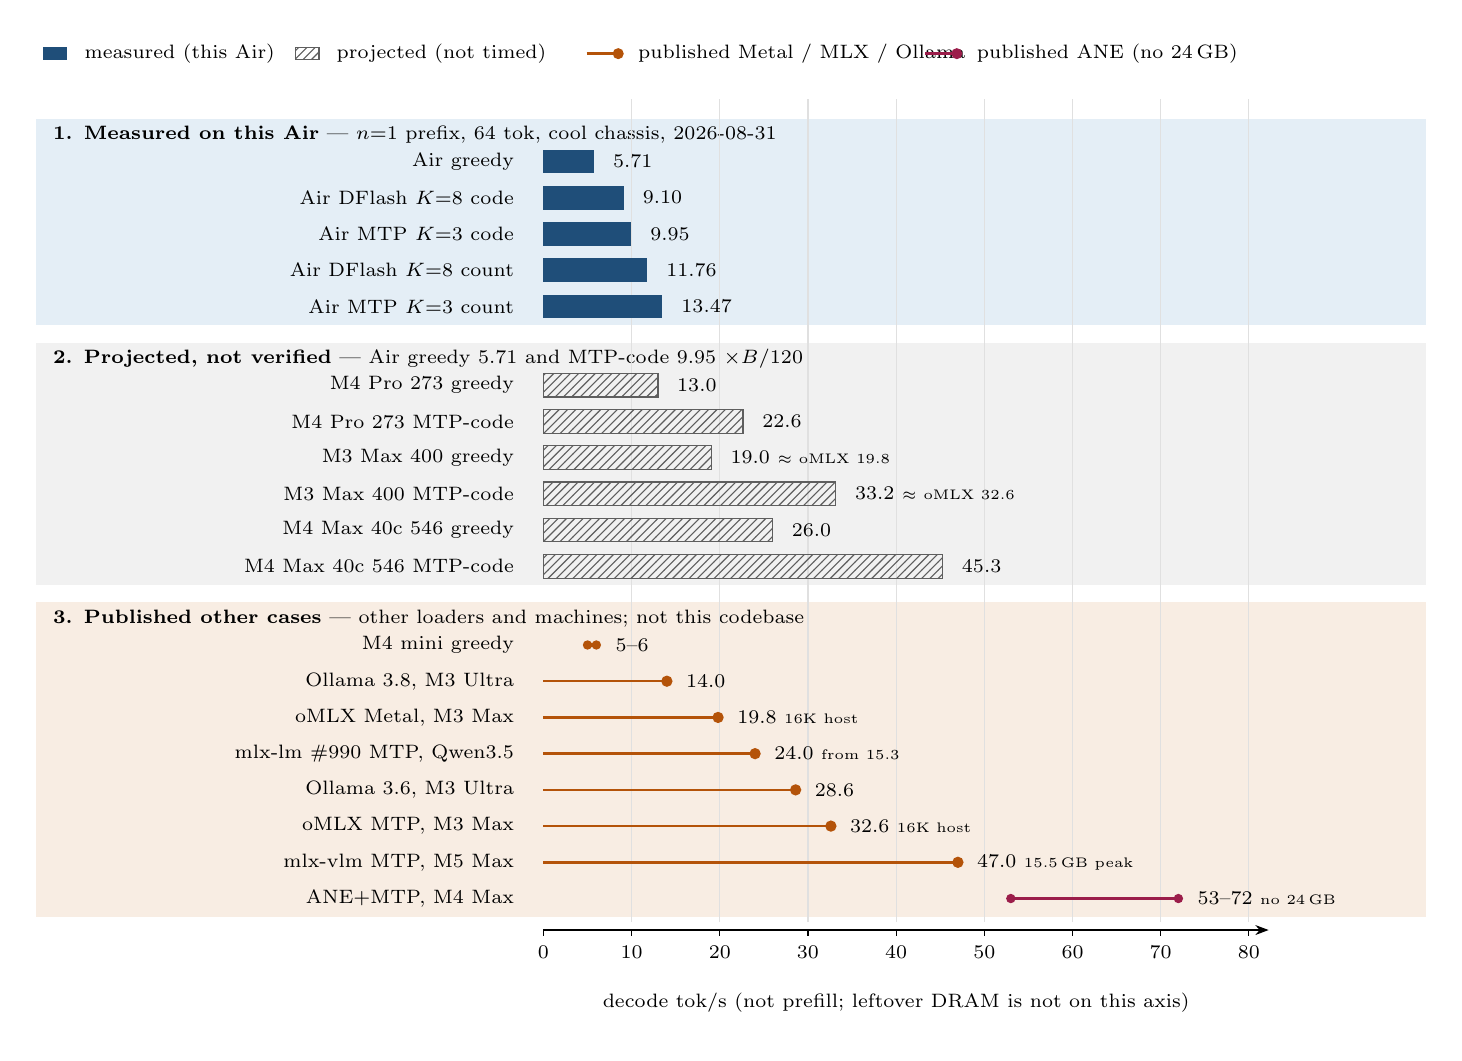
\begin{tikzpicture}[font=\scriptsize, >=Stealth]
\definecolor{meas}{HTML}{1F4E79}
\definecolor{measband}{HTML}{E4EEF6}
\definecolor{proj}{HTML}{5E5E5E}
\definecolor{projband}{HTML}{F1F1F1}
\definecolor{pub}{HTML}{B45309}
\definecolor{pubane}{HTML}{9B1D4A}
\definecolor{pubband}{HTML}{F8EDE3}
\fill[white] (-6.55,-0.85) rectangle (11.310,11.910);
\fill[pubband] (-6.45,0.610) rectangle (11.210,4.610);
\node[anchor=west, font=\scriptsize] at (-6.35,4.410) {{\textbf{3. Published other cases}} --- other loaders and machines; not this codebase};
\fill[projband] (-6.45,4.830) rectangle (11.210,7.910);
\node[anchor=west, font=\scriptsize] at (-6.35,7.710) {{\textbf{2. Projected, not verified}} --- Air greedy 5.71 and MTP-code 9.95 $\times B/120$};
\fill[measband] (-6.45,8.130) rectangle (11.210,10.750);
\node[anchor=west, font=\scriptsize] at (-6.35,10.550) {{\textbf{1. Measured on this Air}} --- $n{=}1$ prefix, 64 tok, cool chassis, 2026-08-31};
\draw[black!12] (1.120,0.55) -- (1.120,11.010);
\draw[black!12] (2.240,0.55) -- (2.240,11.010);
\draw[black!12] (3.360,0.55) -- (3.360,11.010);
\draw[black!12] (4.480,0.55) -- (4.480,11.010);
\draw[black!12] (5.600,0.55) -- (5.600,11.010);
\draw[black!12] (6.720,0.55) -- (6.720,11.010);
\draw[black!12] (7.840,0.55) -- (7.840,11.010);
\draw[black!12] (8.960,0.55) -- (8.960,11.010);
\draw[pubane, line width=1.35pt] (5.936,0.850) -- (8.064,0.850);
\fill[pubane] (5.936,0.850) circle (1.7pt);
\fill[pubane] (8.064,0.850) circle (1.7pt);
\node[anchor=east, align=right] at (-0.25,0.850) {ANE+MTP, M4 Max};
\node[anchor=west] at (8.184,0.850) {53--72 {\tiny no 24\,GB}};
\draw[pub, line width=0.9pt] (0,1.310) -- (5.264,1.310);
\fill[pub] (5.264,1.310) circle (2.05pt);
\node[anchor=east, align=right] at (-0.25,1.310) {mlx-vlm MTP, M5 Max};
\node[anchor=west] at (5.384,1.310) {47.0 {\tiny 15.5\,GB peak}};
\draw[pub, line width=0.9pt] (0,1.770) -- (3.651,1.770);
\fill[pub] (3.651,1.770) circle (2.05pt);
\node[anchor=east, align=right] at (-0.25,1.770) {oMLX MTP, M3 Max};
\node[anchor=west] at (3.771,1.770) {32.6 {\tiny 16K host}};
\draw[pub, line width=0.9pt] (0,2.230) -- (3.203,2.230);
\fill[pub] (3.203,2.230) circle (2.05pt);
\node[anchor=east, align=right] at (-0.25,2.230) {Ollama 3.6, M3 Ultra};
\node[anchor=west] at (3.323,2.230) {28.6};
\draw[pub, line width=0.9pt] (0,2.690) -- (2.688,2.690);
\fill[pub] (2.688,2.690) circle (2.05pt);
\node[anchor=east, align=right] at (-0.25,2.690) {mlx-lm \#990 MTP, Qwen3.5};
\node[anchor=west] at (2.808,2.690) {24.0 {\tiny from 15.3}};
\draw[pub, line width=0.9pt] (0,3.150) -- (2.218,3.150);
\fill[pub] (2.218,3.150) circle (2.05pt);
\node[anchor=east, align=right] at (-0.25,3.150) {oMLX Metal, M3 Max};
\node[anchor=west] at (2.338,3.150) {19.8 {\tiny 16K host}};
\draw[pub, line width=0.9pt] (0,3.610) -- (1.568,3.610);
\fill[pub] (1.568,3.610) circle (2.05pt);
\node[anchor=east, align=right] at (-0.25,3.610) {Ollama 3.8, M3 Ultra};
\node[anchor=west] at (1.688,3.610) {14.0};
\draw[pub, line width=1.35pt] (0.560,4.070) -- (0.672,4.070);
\fill[pub] (0.560,4.070) circle (1.7pt);
\fill[pub] (0.672,4.070) circle (1.7pt);
\node[anchor=east, align=right] at (-0.25,4.070) {M4 mini greedy};
\node[anchor=west] at (0.792,4.070) {5--6};
\fill[pattern=north east lines, pattern color=proj] (0,4.920) rectangle (5.071,5.220);
\draw[proj, thin] (0,4.920) rectangle (5.071,5.220);
\node[anchor=east, align=right] at (-0.25,5.070) {M4 Max 40c 546 MTP-code};
\node[anchor=west] at (5.191,5.070) {45.3};
\fill[pattern=north east lines, pattern color=proj] (0,5.380) rectangle (2.910,5.680);
\draw[proj, thin] (0,5.380) rectangle (2.910,5.680);
\node[anchor=east, align=right] at (-0.25,5.530) {M4 Max 40c 546 greedy};
\node[anchor=west] at (3.030,5.530) {26.0};
\fill[pattern=north east lines, pattern color=proj] (0,5.840) rectangle (3.715,6.140);
\draw[proj, thin] (0,5.840) rectangle (3.715,6.140);
\node[anchor=east, align=right] at (-0.25,5.990) {M3 Max 400 MTP-code};
\node[anchor=west] at (3.835,5.990) {33.2 {\tiny $\approx$ oMLX 32.6}};
\fill[pattern=north east lines, pattern color=proj] (0,6.300) rectangle (2.132,6.600);
\draw[proj, thin] (0,6.300) rectangle (2.132,6.600);
\node[anchor=east, align=right] at (-0.25,6.450) {M3 Max 400 greedy};
\node[anchor=west] at (2.252,6.450) {19.0 {\tiny $\approx$ oMLX 19.8}};
\fill[pattern=north east lines, pattern color=proj] (0,6.760) rectangle (2.535,7.060);
\draw[proj, thin] (0,6.760) rectangle (2.535,7.060);
\node[anchor=east, align=right] at (-0.25,6.910) {M4 Pro 273 MTP-code};
\node[anchor=west] at (2.655,6.910) {22.6};
\fill[pattern=north east lines, pattern color=proj] (0,7.220) rectangle (1.455,7.520);
\draw[proj, thin] (0,7.220) rectangle (1.455,7.520);
\node[anchor=east, align=right] at (-0.25,7.370) {M4 Pro 273 greedy};
\node[anchor=west] at (1.575,7.370) {13.0};
\fill[meas] (0,8.220) rectangle (1.509,8.520);
\node[anchor=east, align=right] at (-0.25,8.370) {Air MTP $K{=}3$ count};
\node[anchor=west] at (1.629,8.370) {13.47};
\fill[meas] (0,8.680) rectangle (1.317,8.980);
\node[anchor=east, align=right] at (-0.25,8.830) {Air DFlash $K{=}8$ count};
\node[anchor=west] at (1.437,8.830) {11.76};
\fill[meas] (0,9.140) rectangle (1.114,9.440);
\node[anchor=east, align=right] at (-0.25,9.290) {Air MTP $K{=}3$ code};
\node[anchor=west] at (1.234,9.290) {9.95};
\fill[meas] (0,9.600) rectangle (1.019,9.900);
\node[anchor=east, align=right] at (-0.25,9.750) {Air DFlash $K{=}8$ code};
\node[anchor=west] at (1.139,9.750) {9.10};
\fill[meas] (0,10.060) rectangle (0.640,10.360);
\node[anchor=east, align=right] at (-0.25,10.210) {Air greedy};
\node[anchor=west] at (0.760,10.210) {5.71};
\draw[->] (0,0.45) -- (9.210,0.45);
\draw (0.000,0.45) -- ++(0,-0.08) node[below, font=\scriptsize] {0};
\draw (1.120,0.45) -- ++(0,-0.08) node[below, font=\scriptsize] {10};
\draw (2.240,0.45) -- ++(0,-0.08) node[below, font=\scriptsize] {20};
\draw (3.360,0.45) -- ++(0,-0.08) node[below, font=\scriptsize] {30};
\draw (4.480,0.45) -- ++(0,-0.08) node[below, font=\scriptsize] {40};
\draw (5.600,0.45) -- ++(0,-0.08) node[below, font=\scriptsize] {50};
\draw (6.720,0.45) -- ++(0,-0.08) node[below, font=\scriptsize] {60};
\draw (7.840,0.45) -- ++(0,-0.08) node[below, font=\scriptsize] {70};
\draw (8.960,0.45) -- ++(0,-0.08) node[below, font=\scriptsize] {80};
\node[anchor=north] at (4.480,-0.22) {decode tok/s (not prefill; leftover DRAM is not on this axis)};
\fill[meas] (-6.35,11.500) rectangle (-6.05,11.660);
\node[anchor=west] at (-5.95,11.580) {measured (this Air)};
\fill[pattern=north east lines, pattern color=proj] (-3.15,11.500) rectangle (-2.85,11.660);
\draw[proj] (-3.15,11.500) rectangle (-2.85,11.660);
\node[anchor=west] at (-2.75,11.580) {projected (not timed)};
\draw[pub, line width=0.9pt] (0.55,11.580) -- (0.95,11.580);
\fill[pub] (0.95,11.580) circle (2pt);
\node[anchor=west] at (1.08,11.580) {published Metal / MLX / Ollama};
\draw[pubane, line width=1.2pt] (4.85,11.580) -- (5.25,11.580);
\fill[pubane] (5.25,11.580) circle (2pt);
\node[anchor=west] at (5.38,11.580) {published ANE (no 24\,GB)};
\end{tikzpicture}

}
\caption{Qwen 27B-class decode, three categories. Solid: this Air. Hatched: unverified $B/120$ cartoons of greedy 5.71 and MTP-code 9.95. Markers: published other cases. ANE 53--72 does not fit 24\,GB. RAM${-}15.1$\,GiB is not plotted.}
\label{fig:bw}
\end{figure}

Table~\ref{tab:27b} and Figure~\ref{fig:bw} keep measured Air pins, bandwidth cartoons, and other people's benches as three encodings. Scaling this Air \emph{up} by $400/120$ predicts 19.0 / 33.2, which sits on oMLX's published 19.8 / 32.6. The M4 Max cartoon is 26.0 / 45.3, not Weschera's ANE 53--72.

A 100-second Monte Carlo (43,097,875 draws, 8\% independent CV) gives $P(\text{ANE }83{\to}274 \ge {+}200\%){=}0.801$, $P(\text{Air MTP} \ge 2\times){=}0.927$, $P(\text{scaled oMLX TG within }4\,\tokspersec\text{ of }9.95){\approx}1$, and zero official-Qwen Mac rows over ${+}200\%$. The official card names SGLang, vLLM, and TokenSpeed and publishes no Mac tok/s table~\citep{qwen38card}. Ollama's ${+}93\%$ is 35B-A3B NVFP4 on M5, 32\,GB+~\citep{ollama019}. Weschera's ${+}230\%$ is ANE prefill on M4 Max 128\,GB~\citep{weschera2026}.

\subsection{Follow-up TTFT class}

When PrefixCache hits, this Air's 819-token reuse is $17.0 \to 0.88$\,s ($19\times$). oMLX reports $7.96\times$ at $\approx 49$k. mlx-engine's template fix reports $25\times$. All three are follow-up clocks. None is a faster first-token QMM.

\subsection{A different model that does hit 30 tok/s}

27B 4-bit cannot hit 30 on 120\,GB/s: a full-pack read is $\approx 8$--10 tok/s, native MTP measured 13.47 / 9.95. Qwen3.5-9B is still GDN-compute-bound here (6.4 raw, 13.8 DFlash). Qwen3.5-4B 4-bit is the pack that clears 30 on this Air (Table~\ref{tab:4b}). 4B finished the same closed task in fewer tokens than 27B. Output is bit-identical to 4B greedy, not to 27B. Daily serve does not swap it in.

\begin{table}[ht]
\centering
\caption{Same Air, thinking and vision off. Qwen3.5-4B is included as a separate pack, not as a 27B drafter.}
\label{tab:4b}
\begin{tabular}{@{}llrl@{}}
\toprule
Pack & Path & tok/s & Peak \\
\midrule
Qwen3.5-4B-4bit & stock mlx-vlm & 32.68 & 2.69\,GiB \\
+ DFlash $K{=}5$ & \texttt{--draft} & 46.39 / 54.32 & 2.87\,GiB \\
Qwen3.5-9B-4bit + DFlash & same & 13.75 & 5.70\,GiB \\
Qwen3.8-27B-4bit + MTP & $K{=}3$ & 13.47 / 9.95 & 14.9--15.1\,GiB \\
Qwen3.8-27B-4bit + DFlash2 & $K{=}8$ & 11.76 / 9.10 & 16.5--17.0\,GiB \\
\bottomrule
\end{tabular}
\end{table}

\subsection{MoE cold start is the number users wait for}

The same $C{=}32$ 35B configuration is 4.2 cold end-to-end to 256 tokens, 6.1 warm sustained decode, and short warm windows reach 6.5--7.8 because a brief burst can run almost entirely out of experts that are already cached. I do not quote the short-window burst as the throughput.

\begin{table}[ht]
\centering
\caption{35B-A3B $C{=}32$, counted from process start. Fixed cost $\approx 19$\,s before the second token.}
\label{tab:moeN}
\begin{tabular}{@{}rrrr@{}}
\toprule
$N$ tokens & Wall from launch & Cold e2e tok/s & Warm decode \\
\midrule
32 & 18.7\,s & 1.71 & 5.5 \\
64 & 32.8\,s & 1.96 & 4.7 \\
128 & 42.1\,s & 3.05 & 5.6 \\
256 & 61.2\,s & 4.19 & 6.07 \\
\bottomrule
\end{tabular}
\end{table}

The same 256 tokens on the pre-\texttt{preadv}, pre-\texttt{memoryview} path took 98\,s at 2.61 cold end-to-end: $1.61\times$ from cold start, $1.88\times$ on decode alone. Short answers see less ($1.20\times$ at 32 tokens) because 19\,s of load and prefill dominate.

llama.cpp at matching Q4 quality cannot run. Five configs: \texttt{-ngl 99} failed to decode the prompt batch (\texttt{res=-3}); \texttt{-ngl 32} hit memory pressure level 4 and was killed; \texttt{-ngl 24} returned \texttt{res=-3}; \texttt{-ngl 99 -c 512 -fa on} hit \texttt{kIOGPUCommandBufferCallbackErrorOutOfMemory}; \texttt{-ngl 99 -ot exps=CPU} again hit pressure 4. UD-IQ4\_XS at 16.29\,GiB would likely fit; that is a smaller, lower-quality quant. The honest claim is that llama.cpp cannot run this model at this quality on this machine.

\subsection{Fanless soak and live OMP}

Cool-machine ceilings are not all-day numbers. After 8--10 minutes the fanless Air sits at roughly 60--70\% of the peak decode rates above. Thinking-on daily serve spends tokens on analysis that the stream holdback then strips from the OMP pane. Live OMP at $T{=}1.0$ is closer to $\approx 10$ tok/s code than the 13.47 greedy-count bench. First pin after boot is $\approx 30$\,s; restarting serve re-pays it. Those are the product clocks. The benches exist so the product clocks have something honest to sit under.

\subsection{Quality of the model versus quality of the serve}

The vendor card (Claude Code harness, $T{=}1.0$) lists 61.7 SWE-bench Pro, 90.3 LiveCodeBench v6, 89.2 GPQA Diamond, and 84.3 OSWorld-Verified. Those rows sit above Qwen3.6-27B on the agent and coding entries, and above Opus~4.6 Max on some software-engineering entries. They are capability scores from a hosted harness, not Mac scores, and they assume a full cloud prompt. Affine-4 is a quality tax; I still treat the local model as the same 27B, not as a new checkpoint. How well that 27B \emph{runs} on this Air is a separate question, taken up in \S\ref{sec:ops}.

\subsection{Envelope suite (structural)}
\label{sec:suite}

Table~\ref{tab:suite} is campaign \texttt{20260902T001357Z}, claim \texttt{C-suite}. All 29 cases kept condensed system $\le 263$ estimator tokens (cap 256${+}8$), a history-stable user dump, and a first-encode prefix that survived follow-up and third turn. The 26k-class dump (8132 raw user tokens) condensed to 1205 first-turn ids; the 39k-class dump (11640 raw) condensed to 1143. Neither refused. Packed length 8192 in the last column is \texttt{keep\_token\_ids} applied to an overlong padded id list---the Metal cap---not the condensed prompt size. Condensed size is \texttt{first\_ids}.

I am not reporting pass@k, SWE-bench, or a side-by-side with the full OMP harness. That comparison is \texttt{C-quality} and needs the 27B plus agent tasks.

\begin{table}[ht]
\centering
\caption{Envelope suite, campaign \texttt{20260902T001357Z}. Token estimates use the campaign's byte-map tokenizer. Representative rows; the full 29 are in \texttt{verification/suite\_latest.json}.}
\label{tab:suite}
{\small
\begin{tabular}{@{}llrrrr@{}}
\toprule
Id & Class & Raw user & Sys tok & Prefix $n$ & First ids \\
\midrule
short-0 & short & 1 & 40 & 162 & 175 \\
file-0 & file & 1007 & 244 & 5002 & 5015 \\
cwd-0 & cwd & 787 & 124 & 560 & 573 \\
cwd-26k & omp-26k & 8132 & 263 & 1192 & 1205 \\
tmp-39k & omp-39k & 11640 & 263 & 1130 & 1143 \\
empty-ask & edge & 0 & 40 & 160 & 172 \\
follow-is-dump & edge & 1509 & 40 & 6194 & 6207 \\
think-tags & edge & 1 & 40 & 162 & 175 \\
\midrule
29 / 29 & all classes & --- & $\le 263$ & $\ge 16$ & packed $\le 8192$ \\
\bottomrule
\end{tabular}
}
\end{table}

%======================================================================
\section{How the Serve Is Run, and How Well That Works}
\label{sec:ops}

The tables in \S\ref{sec:eval} are cool-machine ceilings. This section is the operational review I would give a colleague who asked whether they should leave this process up all afternoon.

\subsection{Process lifetime}

I start serve once and leave it. Pin of the 15\,GiB pack is about 30\,s after boot. \texttt{/models/load} can return after mmap so OMP's spinner stops; the first generate still waits on \texttt{pin()} if I send too early. Restarting serve pays the pin again. I do not treat ``ready'' as ``first token is cheap.''

Admission is \texttt{stored + KV $\le$ total $-$ leave\_free} before load. On 24\,GB the default leave-free of 8\,GiB leaves a 16\,GiB working set, which is not enough for 15\,GiB plus MTP. Daily serve uses 6\,GiB leave-free (18\,GiB WS). That is tight. Safari plus a few Electron windows will still coexist; a Chrome session with a large number of tabs will not. I have jetsamed the machine with a 10k PrefixCache snapshot ($\approx 790$\,MiB extra). The cap is now 2048 tokens / 384\,MiB.

\subsection{What a working day actually feels like}

After 8--10 minutes the fanless chassis sits at roughly 60--70\% of the cool decode rates. That is the number I plan around, not 13.47. Thinking-on daily serve spends tokens on analysis that the stream filter then strips before OMP prints the answer, so wall time per visible token is worse than the greedy bench. Live OMP at temperature 1.0 is closer to 10 tok/s on code than to the 13.47 count-prompt figure. Follow-up turns that hit PrefixCache feel like a different program (0.88\,s vs.\ 17\,s on an 819-token prefix). Turns that edit history, reorder excerpts, or inject the dump log feel like the first turn again.

I advertise a 64k window to OMP so compaction does not loop on a 39k cwd dump. Metal still prefills at most 8192 tokens after the envelope. The 27B does not see the full harness. Cloud OMP still does. That split is the reason a 39k dump is no longer an HTTP 400, and also the reason vendor-card quality numbers do not transfer cleanly.

\subsection{Management surface}

There is no control plane. Management is a small set of files and tests.

\begin{itemize}[leftmargin=1.4em]
\item \texttt{tps.py} is the decision log. Statuses are adopted, attempted, in\_tree, deferred, rejected. \texttt{catalog\_sound()} fails if a banned id is adopted or if the daily draft is no longer sidecar MTP. I added that after I caught myself reopening ANE and 4B-as-drafter every time I wanted more tok/s.
\item \texttt{M4\_AIR\_24G} pins the cool-machine numbers. Tests fail if those drift, or if someone adds an official Qwen Mac tok/s row that the card does not contain.
\item The MLX fence keeps admit, OMP YAML, the context log, and the catalog import-clean. I can reject a bad idea on a Linux VM that has never seen the weights.
\item One directory per local issue for the context log, so two tasks do not share a cache key.
\item Serve writes static \texttt{llama.cpp} / \texttt{lm-studio} rows into \texttt{\~/.omp/agent/models.yml} without loading weights. I refresh OMP models after that, then wait for \texttt{ready}.
\end{itemize}

I would not call this ``orchestration.'' It is closer to a lab notebook that happens to be executable. The cost of that choice is that there is no multi-user scheduler, no second replica, and no way to move prefill off the Air. The benefit is that the policy I think I am running is the policy the tests compile.

\subsection{Judgement}

I would describe the arrangement as: the 27B is good enough for agent and code work that I would otherwise send to a hosted API; it fits if I stay on 4-bit and leave-free 6g; it is slow in the way 120\,GB/s and 10 GPU cores are slow. Cool greedy decode is 5.71 tok/s. Cool MTP is 9.95--13.47 depending on the prompt. Prefill of a fresh 819-token body is 17\,s. A true prefix follow-up is under a second. After a soak those decode rates sag. First pin is half a minute. That is usable for interactive coding if I keep serve up and if I accept that the model sees a condensed harness. It is a poor substitute for a Max if the job is long-context prefill or a demo that needs 40 tok/s on camera.

The 35B-A3B path is in a different category. llama.cpp at matching Q4 quality did not run. Stock mlx-lm thrashed. $C{=}32$ produced 4.2 cold end-to-end tok/s to 256 tokens and 6.1 warm. That is ``the model exists on this RAM,'' not something I would use as a daily coder. I leave it in the report because it is the original reason the slot pack exists, and because the $C$-sweep is the cleanest evidence I have that unified memory is not a discrete GPU with a nicer name.

%======================================================================
\section{What Is Assembled and What I Had to Invent}
\label{sec:unique}

Most of the parts are ordinary. MTP is Qwen's. Rejection sampling is Leviathan--Chen. Fused Metal GDN is MLX's. The 4-bit packs are community checkpoints. Prefix caching is old. Every production proxy has some kind of envelope. Leave-free is just a working-set reserve with a macOS-shaped name.

What I have not seen written down as a 24\,GB Air recipe---and I may have missed a gist---is the combination below. I am not claiming each mechanism is original in isolation.

\paragraph{Prefix cache vs.\ Qwen's template.}
LM Studio and others found the think-tag miss~\citep{qwen31826,mlxengine176} and patched Jinja. I left the stock template alone and snapped at the common prefix of two \texttt{apply\_chat\_template} calls, one with the generation prompt and \texttt{/no\_think} and one without. History and last-ask use the same condense recipe. The dump log is not compiled back into the system prefix unless I set a flag. Restore writes \texttt{KVCache.offset} from the key length when the setter leaves 0~\citep{mlxlm1162}.

\paragraph{Envelope that does not rewrite OMP.}
The usual local proxies either send the whole prompt or change the agent's system text. I kept a third copy: OMP still has the harness, Metal sees 256 tokens of it, disk has the verbatim dump. Follow-up PrefixCache hits depend on that split. The 27B is not seeing what the cloud agent sees. I treat that as a product choice with a quality cost, not as a free compression.

\paragraph{Pyramid on ids.}
PyramidKV compresses KV~\citep{pyramidkv}. I used the same keep-set shape (sink, sparse middle, tail) as an admission policy for which token ids get prefills. Applying it to GDN state would be a different model. I say this only because I almost did it once.

\paragraph{Catalog of refusals.}
Related-work sections do not usually fail CI. \texttt{catalog\_sound()} does, if ANE or 4B-as-drafter gets marked adopted. I added it after I reopened both of those in the same week.

\paragraph{Slots that turn off.}
Expert caches on discrete GPUs are common. This one is sized so the rest of the bank can stay in the page cache, and \texttt{install\_expert\_slots} is a no-op on dense modules. I did not layer-stream a 27B that already fits at 4-bit.

\paragraph{Import fence.}
I kept admit, OMP, context, and the catalog free of MLX so I can test the policy on a machine that cannot pin 15\,GiB. The Linux workspace that compiled this PDF is that machine.

I also keep three identity claims separate, because collapsing them is how a wrapper becomes a different model. Default MoE decode matched stock mlx-lm (maxabs 0.0). The preadv path is tested to land rows at the recorded pack offsets. Dense speculation matches the 27B only because verify is Leviathan--Chen through a rollback that can rewind GDN.

\subsection{Published levers I did not take}

Table~\ref{tab:non} lists accelerations I was asked about, or that I considered, and did not put on the daily door. Each has a published number. Each breaks a constraint in \S\ref{sec:intro} on this machine.

\begin{table}[t]
\centering
\caption{Accelerations I considered or was asked about, and did not put on the daily 27B door.}
\label{tab:non}
\begin{tabular}{@{}p{3.4cm}p{4.2cm}p{5.6cm}@{}}
\toprule
Lever & Published claim & Why not here \\
\midrule
oMLX ANE prefill & $83{\to}274$ tok/s (${+}230\%$) & Second copy, 64--128\,GB, private ANE \\
Ollama MLX 0.19 & ${+}93\%$ decode & 35B-A3B, 32\,GB+, M5 \\
CUDA chunked GDN & $8.5\times$ TTFT & Metal already fused; chunked slower on M \\
SpecPrefill / SwiftKV & $2$--$7\times$ TTFT & Changes prompt or weights \\
DistServe P/D & cluster goodput & One worker; arrays cannot cross threads \\
4B as 27B drafter & classic spec & Wrong width; trim path; RAM \\
KV-quant + draft & memory & Verifier reads \texttt{keys.shape} \\
Hybrid KV page & ``fit 128k'' & Cannot trim GDN; changes text if faked \\
MTP+DFlash together & stacked spec & One verify, DFlash already lost \\
Forced $K{=}5$ & one knob & Wrong trained length for both students \\
\bottomrule
\end{tabular}
\end{table}

%======================================================================
\section{Failure Modes and Threats to Validity}
\label{sec:threats}

The following are ways the 27B door has been wrong, slow, or incomparable, including bugs I already closed. I include them because the happy-path tables are otherwise too clean.

\subsection{Silent wrongness (the class this runtime exists to refuse)}

\begin{enumerate}[leftmargin=1.4em]
\item \textbf{mlx-lm trim speculation on ArraysCache.} Rejected drafts remain in $S_t$. No exception. Banned; daily path is mlx-vlm rollback.
\item \textbf{T${>}1$ chunked GDN verify.} $\approx 4\%$ argmax flips vs.\ $T{=}1$. Not used as a ``cheap verify.''
\item \textbf{KV-quant with draft.} Verifier reads \texttt{keys.shape}; quant changes the tensor the rollback inspects. Forced off when a draft is set.
\item \textbf{Vocab / width mismatch.} Qwen3 151936 vs.\ Qwen3.5/3.8 248320; 4B hidden $\approx 2560$ vs.\ 5120. A family-name drafter is a different model.
\item \textbf{DAIS persist.} Low-accept think dumps left the next ``hi'' at $K{=}1$. Reset every request.
\item \textbf{Session offset past EOS.} DFlash can accept past stop; attention offset runs ahead of fed ids. Cache dropped unless every attention layer matches $|\mathrm{fed}|$.
\item \textbf{Waves / split-K.} Optional prefill waves change logits. Off by default.
\item \textbf{Pyramid on GDN.} Compressing recurrent state is a different (wrong) model. Pyramid is applied to ids only.
\end{enumerate}

\subsection{Silent slowness (correct tokens, wasted forwards)}

\begin{enumerate}[leftmargin=1.4em]
\item \textbf{Qwen generation prompt.} Empty think tags and last-ask \texttt{/no\_think} are not prefixes of the next encode. Snap at the dual-template body.
\item \textbf{Context-OS inject of the dump log.} Newest-first compile is a new key every turn. Inject off unless explicitly requested.
\item \textbf{Last-user-only condense.} History recipe differed from last-ask recipe; \texttt{ids[:n]} missed. Same recipe every user dump.
\item \textbf{Geometric crumbs at 256/512/1024.} Split the first 2k of an 8k envelope into extra 27B forwards. Eviction already dropped them first; they are gone.
\item \textbf{Hardcoded snap 128.} Split every short ``hi'' into two forwards.
\item \textbf{KV offset left at 0 on restore.} Suffix appended onto an empty-looking cache (mlx-lm\#1162 class). Restore writes offset from key length.
\item \textbf{Full-prompt mRoPE prime.} Wrote deltas the step then nulled; on an 8k envelope that was a discarded full-prompt rope index.
\item \textbf{Per-chunk eval+clear.} Server-vs-vMLX TTFT gap on the same Mac. One terminal eval.
\item \textbf{512\,MiB allocator during a large tile.} Per-layer Metal malloc (mlx\#3350). Prefill raises to 2\,GiB, then restores 512.
\item \textbf{\texttt{.item()} after eval.} $40\times 224\,\mu\mathrm{s}$/token on the MoE path. \texttt{memoryview}.
\end{enumerate}

\subsection{Threats to validity}

\paragraph{External.} One fanless Air. Bandwidth scaling of Max numbers matches decode here; it does not prove the next M-series chip will sit on the same line. Published Mac benches mix Ollama, llama.cpp, oMLX, mlx-lm, and mlx-vlm; they are cited as named clocks, not as a meta-average.

\paragraph{Internal.} Page-cache state is a confounder on every MoE A/B. Cool-vs-soak is a confounder on every 27B decode number. Thinking-on vs.\ thinking-off changes tokens emitted, not just tok/s. Envelope lossiness means the 27B does not see the full OMP harness; quality numbers from the vendor card assume a cloud prompt.

\paragraph{Construct.} ``Fits'' means admit plus a generate that does not jetsam, not ``comfortable multitasking.'' ``Exact verify'' means Leviathan--Chen through mlx-vlm rollback, not bitwise identity of Metal reductions across mlx-lm vs.\ mlx-vlm graph shapes. ``Unique'' means we have not seen the same intersection published as a 24\,GB Air recipe; it does not mean no component exists elsewhere.

\paragraph{Statistical.} The Monte Carlo on the ${+}200\%$ claim stresses published point estimates under an assumed 8\% CV. It is not a new bench, and a reviewer who discarded it would be within their rights. The 27B MTP vs.\ DFlash comparison is a matched pair on one prefix, not a 50-prompt sweep. The MoE $C$-sweep is two cold reps plus an alternating warm A/B: enough to see an interior optimum, not enough for a confidence interval.

\paragraph{Verification coverage.} Campaign \texttt{20260902T001357Z} reproduced the twenty-one \texttt{verified\_here} claims and pin-checked the two Air clocks. That is software and arithmetic, not a new Metal bench. The envelope suite ($n{=}29$) is a structural oracle on a deterministic tokenizer stand-in; it does not estimate task quality. A reviewer who asked for multi-machine results, a 50-prompt Metal sweep, and an ablation of envelope quality against the full OMP harness (\texttt{C-quality}) would be asking for work I have not done. The operational claims in \S\ref{sec:ops} are from one person's daily use on one fanless Air, and soak remains \texttt{C-soak}.

%======================================================================
\section{Limitations}
\label{sec:limit}

\paragraph{Silicon.} 10 GPU cores and 120\,GB/s will not become a Max. MTP $2.36\times$ is the transferable half of the 2026 Mac story. ANE is not.

\paragraph{First request.} Pin is $\approx 30$\,s. Returning ready after mmap only stops the OMP spinner; the first generate still waits.

\paragraph{Cold prefill.} 48 tok/s on 15\,GiB is the remaining honest hole. In-tree questions: PrefixCache restore vs.\ GDN/KV positions (partially repaired), \texttt{generate\_step} after \texttt{skip\_logits} tiles, and QMM as the compute floor. This VM cannot retime Metal 27B.

\paragraph{Quality.} 4-bit is not bf16. Thinking-on daily serve spends tokens. OMP $T{=}1.0$ lowers accept vs.\ the greedy bench.

\paragraph{Envelope lossiness.} The 27B does not see the full harness. Cloud OMP still does. Context OS keeps the bytes on disk; the model sees a budgeted extract. Quality claims that assume the cloud prompt do not carry over.

\paragraph{MoE speed.} 6 tok/s warm on 35B-A3B is ``runs,'' not ``snappy.'' The contribution is existence at this quality on this RAM.

\paragraph{Scope.} No CUDA, no Windows, no Intel Mac, no multi-GPU, no GUI.

%======================================================================
\section{Conclusion}
\label{sec:conc}

I set out to run two things on one 24\,GB Air: MoE banks that do not fit in the Metal working set, and a hybrid 27B that I was not willing to speculate or prefix-cache by trimming recurrent state. The daily 27B setup is small. Affine-4 in 18\,GiB. MTP verified by a kernel that can roll GDN back. Snapshots only of exact prefixes, at a Qwen-stable boundary, under 2048 tokens. An envelope that condenses the harness without editing OMP. A catalog that fails tests if I mark a refused idea as adopted. MLX confined to three files so the rest can be checked without the weights. A campaign log that says, for each claim, whether this host reproduced it, pinned it, or cannot retime it.

On this machine that produces about 6 tok/s greedy, 10--13.5 with MTP on a cool chassis, about 48 tok/s on a cold 819-token prefill, and a $19\times$ follow-up when the next encode really is a prefix. Those decode rates are close to a 120/400 scaling of published M3 Max Metal numbers. They are not close to 40--70 tok/s screenshots from Max and Ultra boxes. I think that is the correct reading of the bandwidth, not a missing flag. Campaign \texttt{20260902T001357Z} does not change those clocks. It stops me from writing as if I had retimed them on the machine that compiled the PDF.

\section*{Acknowledgements}

I thank the mlx-lm, mlx-vlm, oMLX, Ollama, and Qwen authors for the kernels, packs, and published benches I relied on. Errors in interpretation, and all Air measurements, are mine.

\bibliographystyle{plainnat}
\bibliography{refs}

\appendix
\section{Catalogued strategies}
\label{app:catalog}

Statuses as of 2 September 2026. Adopted routes may not set trim-cache or target-weight-change flags. The table is the fail-closed catalog, not a backlog. Claim \texttt{C-catalog} fails if a banned id is marked adopted.

{\small
\begin{longtable}{@{}p{4.0cm}lp{8.4cm}@{}}
\toprule
Id & Status & One-line \\
\midrule
\endfirsthead
\toprule
Id & Status & One-line \\
\midrule
\endhead
sidecar-mtp-k3 & adopted & Native MTP $K{=}3$, exact verify \\
auto-sidecar-mtp & adopted & Attach sibling MTP if \texttt{--draft} omitted \\
dais-trained-cap & adopted & Never exceed trained $K$ \\
dais-reset-each-request & adopted & Trained $K$ every request \\
draft-prefix-cache & adopted & Exact snaps on the MTP path \\
suffix-prefix-reuse & adopted & Prefill only the appended suffix \\
qwen-chat-prefix-stable & adopted & Snap pre-\texttt{/no\_think} body \\
omp-reencode-prefix & adopted & Same condense; no log inject; fix offset \\
omp-cold-prefill-n & adopted & 256-token system; 2\,GiB prefill pool \\
async-prefill-pipeline & adopted & async\_eval tiles; one clear \\
skip-lm-head-prefill & adopted & \texttt{skip\_logits} on tiles \\
ttft-is-prefill & adopted & TTFT is GDN prefill, not MTP \\
omp-serve-envelope & adopted & Condense, slim, pack, 8k \\
omp-session-vs-metal & adopted & OMP 64k bar; Metal 8k \\
qwen-no-think-prompt & adopted & \texttt{/no\_think} + holdback \\
harness-temp-1 & adopted & Keep $T{=}1.0$; remap locally \\
omp-models-yml & adopted & Static picker rows \\
omp-defer-weight-pin & adopted & Ready after mmap; pin after \\
skip-vlm-rope-prime & adopted & Do not full-prompt mRoPE \\
context-os & adopted & Disk log + verbatim excerpts \\
vlm-rollback & in\_tree & mlx-vlm rewind of GDN on reject \\
igpu-pyramid-tiles & in\_tree & Pack geometry on ids \\
two-stage-harness & in\_tree & Cloud full; local condensed \\
prompt-lookup & in\_tree & Inert: needs trim \\
dflash2-k8 & attempted & Slower and heavier than MTP \\
mtplx-engine & deferred & 32\,GB+; unmeasured brew \\
tree-medusa-eagle & deferred & Extra kernels; GDN trees \\
leap-mtp & deferred & No L-MTP ckpt here \\
vllm-gdn-block-apc & deferred & Kernel does not return $h$ \\
gdn-cache-contiguous & deferred & Slice leak class \\
metal-qmm-prefill & deferred & Affine-4 floor; no requant \\
warm-prefix-at-load & deferred & Dummy miss is a 17\,s tax \\
ane-npu-prefill & rejected & Second copy; 24\,GB \\
qwen-mac-200pct & rejected & Headline is ANE on 128\,GB \\
gdn-chunked-cuda-prefill & rejected & Metal already fused \\
spec-prefill-sparse & rejected & Changes prompt/weights \\
distserve-pd & rejected & One worker \\
qwen35-4b-as-27b-drafter & rejected & Different model \\
mtp-plus-dflash & rejected & One verify \\
forced-k5 & rejected & Wrong trained $K$ \\
hybrid-kv-dynamic-page & rejected & Cannot trim GDN \\
kv-quant-with-draft & rejected & \texttt{keys.shape} \\
pflash-drop-prompt & rejected & Changes prompt \\
reverse-spec-small-writer & rejected & 4B writes tokens \\
unquantized-bf16-27b & rejected & Does not fit \\
layer-stream-gdn & rejected & 1 tok/s path \\
async-metal-queues & rejected & Arrays cannot cross threads \\
skip-full-attn-on-draft & rejected & Changes draft \\
extra-quant-3bit & rejected & New checkpoint \\
harness-structure-for-tps & rejected & Does not raise GEMM \\
sliding-window-kv & rejected & Changes 27B text \\
named-kv-survey & rejected & Research-only \\
\bottomrule
\end{longtable}
}

\section{Source map}
\label{app:source}

The paper's claims are pinned to these artifacts. Paths are relative to the repository root.

\begin{center}
\small
\begin{tabular}{@{}p{4.4cm}p{8.8cm}@{}}
\toprule
Artifact & What it encodes \\
\midrule
\texttt{src/slotbank/tps.py} & Catalog, \texttt{M4\_AIR\_24G}, Mac-claim runs, \texttt{catalog\_sound}, \texttt{review\_mac\_speedup} \\
\texttt{src/slotbank/runtime.py} & PrefixCache, tiles, draft arming, mlx-vlm generate \\
\texttt{src/slotbank/expert\_slots.py} & Steal / remap / fill / freeze; preadv into pack \\
\texttt{src/slotbank/offload\_cache.py} & File bank, layout, mmap/pread \\
\texttt{src/slotbank/prompt.py} & Condense, slim tools, pyramid ids, \texttt{/no\_think} \\
\texttt{src/slotbank/omp.py} & Static picker rows; MLX-free \\
\texttt{src/slotbank/context\_os.py} & Append-only log; verbatim compile \\
\texttt{src/slotbank/admit.py} & Leave-free working set; MLX-free \\
\texttt{src/slotbank/decode.py} & Sampler / holdback; may use \texttt{os}, not MLX \\
\texttt{docs/mlx-lm-speculative-bug.md} & Silent trim no-op \\
\texttt{tests/test\_fence.py} & Only three files import MLX (\texttt{C-fence}) \\
\texttt{tests/test\_tps.py} & Catalog and Mac-claim invariants \\
\texttt{tests/paper\_claims.py} & Claim registry, RQs, optional-dep names \\
\texttt{tests/test\_paper\_verification.py} & One test per claim; envelope suite \\
\texttt{scripts/verify\_paper.py} & Dated campaign writer \\
\texttt{verification/campaign\_latest.md} & Traceability log (kind, test, status) \\
\texttt{README.md} & MoE benches, $C$-sweep, I/O phases \\
\bottomrule
\end{tabular}
\end{center}

\section{Claim matrix}
\label{app:claims}

Campaign \texttt{20260902T001357Z}. Kind and status are defined in \S\ref{sec:verify}. The same rows are \texttt{tests/paper\_claims.py}.

{\small
\begin{longtable}{@{}llllp{6.6cm}@{}}
\caption{Claim registry. Kind is the allowed sentence; status is campaign \texttt{20260902T001357Z}.}
\label{tab:claims}\\
\toprule
Id & RQ & Kind & Status & Statement \\
\midrule
\endfirsthead
\toprule
Id & RQ & Kind & Status & Statement \\
\midrule
\endhead
\texttt{C-fence} & RQ4 & verified & verified & Only three files import MLX. \\
\texttt{C-catalog} & RQ4 & verified & verified & Banned ids cannot be adopted; adopted routes keep 27B text. \\
\texttt{C-clocks} & RQ1 & air pin & pin-checked & 5.71 greedy; 13.47/9.95 MTP; 11.76/9.10 DFlash; 17.0s/0.88s prefill. \\
\texttt{C-pack-ceil} & RQ1 & verified & verified & 4-bit pack-read ceiling on 120\,GB/s is in $[7,9]$. \\
\texttt{C-mac200} & RQ1 & verified & verified & No official Qwen Mac tok/s row; ${+}200\%$ hit is ANE prefill. \\
\texttt{C-scale} & RQ1 & verified & verified & oMLX $\times 120/400$ is 5.94 / 9.78, near the Air pins. \\
\texttt{C-hybrid-kv} & RQ2 & verified & verified & Full-attn KV is 64\,KiB/token; trim path refused. \\
\texttt{C-trained-k} & RQ2 & verified & verified & Draft block is trained $K$ (MTP 3, DFlash 8). \\
\texttt{C-leave-free} & RQ3 & verified & verified & Default leave-free 8\,GiB; 27B door needs 6\,GiB (18\,GiB WS). \\
\texttt{C-slots-c} & RQ3 & verified & verified & 35B-A3B $C \in (16,256)$; OLMoE stays at the $2\times$top-$k$ floor. \\
\texttt{C-sys-cap} & RQ5 & verified & verified & System head is 256 tokens on every turn. \\
\texttt{C-history} & RQ5 & verified & verified & User-dump condense matches last-ask and history. \\
\texttt{C-prefix} & RQ5 & verified & verified & Follow-up encode shares \texttt{stable\_prefix\_n}. \\
\texttt{C-pack-8k} & RQ5 & verified & verified & After envelope, Metal ids $\le 8192$; 26k/39k do not refuse. \\
\texttt{C-pyramid} & RQ5 & verified & verified & \texttt{keep\_token\_ids} is sink + pyramid + tail; 8k head is 2048. \\
\texttt{C-slim} & RQ5 & verified & verified & Slim tools drop JSON schemas; stay in the 256-token budget. \\
\texttt{C-inject} & RQ5 & verified & verified & Serve does not compile \texttt{CONTEXT\_DIR} unless inject${=}1$. \\
\texttt{C-context} & RQ5 & verified & verified & Log is append-only; compile is newest verbatim spans. \\
\texttt{C-session} & RQ2 & verified & verified & \texttt{dflash\_session\_ok} refuses attention offset past $|\mathrm{fed}|$. \\
\texttt{C-sampling} & RQ2 & verified & verified & $T\ge 0.99$ remaps to Qwen's instruct pair; $T<0.99$ is left. \\
\texttt{C-suite} & RQ5 & verified & verified & 29/29 cases keep system, pack, and prefix invariants. \\
\texttt{C-quality} & RQ5 & gap & documented & Task quality of 8k vs.\ full OMP harness. \\
\texttt{C-soak} & RQ1 & gap & documented & Fanless soak 60--70\% after 8--10 min. \\
\texttt{C-metal-toks} & RQ1 & air pin & pin-checked & Live Metal 27B tok/s; this VM has no weights. \\
\bottomrule
\end{longtable}
}

\section{Daily serve contract}
\label{app:serve}

\begin{verbatim}
PYTHONPATH=src .venv/bin/python -m slotbank.cli serve \
  --model ~/Models/Qwen3.8-27B-4bit \
  --leave-free 6g --thinking --vision --direct
\end{verbatim}

Sibling \texttt{Qwen3.8-27B-MTP-4bit} is auto-attached. Point OMP at \texttt{http://127.0.0.1:8080}. Run \texttt{omp models refresh}. Wait for \texttt{ready}. First pin is $\approx 30$\,s; keep serve running.

\section{Notation}
\label{app:notation}

\begin{center}
\begin{tabular}{@{}ll@{}}
\toprule
Symbol & Meaning \\
\midrule
$C$ & Resident expert slots \\
$K$ & Speculative block (trained 3 or 8) \\
$B$ & Delivered bandwidth of the serving tier \\
$W_{\mathrm{touch}}$ & Bytes read per token \\
$s_t$ & GDN recurrent state after token $t$ \\
$f$ & Fed token ids (prompt + generated) \\
$x$ & New request token ids \\
$A$ & Accepted extra draft tokens \\
$\alpha_i$ & Leviathan--Chen accept probability of draft $i$ \\
$S_t$ & GDN matrix state after token $t$ \\
\bottomrule
\end{tabular}
\end{center}

\section{Report descriptors (checklist)}
\label{app:desc}

A reader reproducing or citing this work should record at least:

\begin{enumerate}[leftmargin=1.4em]
\item Machine: chip, unified RAM, advertised Metal WS, measured or published bandwidth.
\item Checkpoint: repo id, quant (affine-4 vs.\ mixed 3.5 vs.\ GGUF), MTP/DFlash sibling, vision tower present or not.
\item Loader: mlx-lm vs.\ mlx-vlm vs.\ oMLX vs.\ llama.cpp vs.\ Ollama. Rollback primitive if any.
\item Leave-free / working set. Admit decision (stored + KV $\le$ total $-$ leave\_free).
\item Envelope: system-token cap, tool slim, id-pack cap, advertised vs.\ Metal window.
\item Sampler: temperature, top-$p$, top-$k$, thinking on/off. OMP $T{=}1.0$ is not greedy.
\item Clock: cold e2e / warm decode / TTFT / follow-up TTFT / compute-only. $N$ tokens. Cool vs.\ soak.
\item Cache: PrefixCache hit/miss, snap length, whether history was edited.
\item Draft: kind, trained $K$, whether $K$ was reset this request, KV-quant on or off.
\item Correctness oracle: bit-match against which greedy baseline, or ``not claimed.''
\item Campaign id from \texttt{verification/campaign\_latest.md}. Kind of each cited claim (\texttt{verified\_here} / \texttt{air\_pinned} / \texttt{cannot\_retime}).
\end{enumerate}

\end{document}
